\documentclass[output=paper,colorlinks,citecolor=brown,draft]{langscibook}
\ChapterDOI{10.5281/zenodo.10641187}
\title[Noun phrase modifiers in early Germanic languages] {Noun phrase modifiers in early Germanic: A comparative corpus study of Old English, Old High German, Old Icelandic, and Old Saxon} 

\abstract{This chapter gives an overview of modifier position in noun phrases in the early Germanic languages Old English, Old High German, Old Icelandic, and Old Saxon. We first present data for the relative position of adjectives, cardinal numerals, possessives, participles, and quantifiers in relation to the head noun. Then we compare aspects of the different languages and discuss factors that might account for the distribution, such as texts and genres, weight, and lexical factors. We show that the default position for modifiers in early Germanic languages is prenominal, and that instances of postnominal modification in most cases can be explained with reference to specific factors. Because the evidence for default prenominal modification is so clear in these languages, we question whether noun phrase modification was ever by default, or even mostly, postnominal in Proto-Germanic, despite the evidence from Runic data and early Gothic, which shows adjectives in postnominal position.}


\author{Kristin Bech\orcid{}\affiliation{University of Oslo} and Hannah Booth\orcid{}\affiliation{Ghent University} and Kersti Börjars\orcid{}\affiliation{University of Oxford} and Tine Breban\orcid{}\affiliation{The University of Manchester} and Svetlana Petrova\orcid{}\affiliation{Bergische Universität Wuppertal} and George Walkden\orcid{0000-0001-5950-9686}\affiliation{University of Konstanz}}


\IfFileExists{../localcommands.tex}{
   \addbibresource{../localbibliography.bib}
   \usepackage{langsci-optional}
\usepackage{langsci-gb4e}
\usepackage{langsci-lgr}

\usepackage{listings}
\lstset{basicstyle=\ttfamily,tabsize=2,breaklines=true}

%added by author
% \usepackage{tipa}
\usepackage{multirow}
\graphicspath{{figures/}}
\usepackage{langsci-branding}

   
\newcommand{\sent}{\enumsentence}
\newcommand{\sents}{\eenumsentence}
\let\citeasnoun\citet

\renewcommand{\lsCoverTitleFont}[1]{\sffamily\addfontfeatures{Scale=MatchUppercase}\fontsize{44pt}{16mm}\selectfont #1}
  
   %% hyphenation points for line breaks
%% Normally, automatic hyphenation in LaTeX is very good
%% If a word is mis-hyphenated, add it to this file
%%
%% add information to TeX file before \begin{document} with:
%% %% hyphenation points for line breaks
%% Normally, automatic hyphenation in LaTeX is very good
%% If a word is mis-hyphenated, add it to this file
%%
%% add information to TeX file before \begin{document} with:
%% %% hyphenation points for line breaks
%% Normally, automatic hyphenation in LaTeX is very good
%% If a word is mis-hyphenated, add it to this file
%%
%% add information to TeX file before \begin{document} with:
%% \include{localhyphenation}
\hyphenation{
affri-ca-te
affri-ca-tes
an-no-tated
com-ple-ments
com-po-si-tio-na-li-ty
non-com-po-si-tio-na-li-ty
Gon-zá-lez
out-side
Ri-chárd
se-man-tics
STREU-SLE
Tie-de-mann
}
\hyphenation{
affri-ca-te
affri-ca-tes
an-no-tated
com-ple-ments
com-po-si-tio-na-li-ty
non-com-po-si-tio-na-li-ty
Gon-zá-lez
out-side
Ri-chárd
se-man-tics
STREU-SLE
Tie-de-mann
}
\hyphenation{
affri-ca-te
affri-ca-tes
an-no-tated
com-ple-ments
com-po-si-tio-na-li-ty
non-com-po-si-tio-na-li-ty
Gon-zá-lez
out-side
Ri-chárd
se-man-tics
STREU-SLE
Tie-de-mann
}
   \boolfalse{bookcompile}
   \togglepaper[3]%%chapternumber
}{}

\lehead{K. Bech, H. Booth, K. Börjars, T. Breban, S. Petrova \& G. Walkden}
\begin{document}
\maketitle
\lehead{K. Bech, H. Booth, K. Börjars, T. Breban, S. Petrova \& G. Walkden}
\section{Introduction}\label{intro}
The present study provides an overview and discussion of the general \isi{noun} phrase \isi{modification} patterns in four old \ili{Germanic} languages: Old \ili{English}, Old High \ili{German}, \ili{Old Icelandic}, and \ili{Old Saxon}. The \ili{Germanic} languages stem from Proto-\ili{Germanic}, one branch of the \ili{Indo-European} family of languages. There is no one agreed approach to the dating and naming of the earliest periods of \ili{Germanic}. It is generally agreed that the earliest runic remains\footnote{The oldest rune stone is the Svingerud stone, discovered in the autumn of 2021, near Oslo, Norway, and revealed to the world in January 2023. It dates from between 1 and 250 CE.} are of a North-West \ili{Germanic} language, which had started to develop separately from East \ili{Germanic}, and which later developed into Common \ili{Scandinavian} (North \ili{Germanic}) and West \ili{Germanic}, each developing sub-divisions over time. As for the East \ili{Germanic} branch, \ili{Gothic} is the only language for which we have fairly robust evidence \citep[with particular relevance to the topic of this chapter, see][]{ratkus2011}. In our study, \ili{Old Icelandic} represents North \ili{Germanic}, whereas Old \ili{English}, Old High \ili{German}, and \ili{Old Saxon} represent West \ili{Germanic}. 

The four languages we investigate stem from different time periods. Old \ili{English} and Old High \ili{German} cover the period from approximately 700 to 1100, while \ili{Old Saxon} is mainly attested in 9\textsuperscript{th} century texts. \ili{Old Icelandic} is the “youngest” of the languages in terms of written sources, with written material, apart from runes, primarily from the 13\textsuperscript{th} century onwards. However, \ili{Old Icelandic} was spoken for a long time before that, and generally covers the period from the 7\textsuperscript{th} to the 15\textsuperscript{th} century. 

The question therefore arises as to whether these languages are comparable. Here we take recourse to Lass’s \citeyearpar{Lass00} proposal that different \ili{Germanic} languages reflect different stages in the development away from their common ancestor. For example, \ili{Gothic} and \ili{Old Icelandic} are ranked as being “oldest”, i.e. closest to their common ancestor, with Old \ili{English} in second place, followed by Old High \ili{German} \citeyearpar[30]{Lass00}. \ili{Old Saxon} is not part of Lass’s ranking scale, but it patterns with Old \ili{English} in having the same archaic features. The ranking is based on linguistic criteria\footnote{The linguistic criteria are: root-initial accent, at least three distinct vowel qualities in weak inflectional syllables, a \isi{dual}, grammatical gender, four vowel-grades in (certain) strong verbs, distinct \isi{dative} in at least some nouns, inflected definite \isi{article} (or proto-\isi{article}), \isi{adjective} \isi{inflection}, infinitive suffix, and person/number marking on the verb.} \citeyearpar[26]{Lass00}, and is thus independent of manuscript production dates. Our assumption is that the four languages of this study all represent an “old” stage.

\section{Background}\label{sectbackground}

The point of departure for the study was the reported divergence in the literature on what the canonical order is for modifier and \isi{noun} in the languages. 

It is generally recognized that substantial changes have taken place in the \ili{Germanic} languages with respect to their organizational principles. The changes have traditionally been described as a development from relatively free \isi{word order} to a more rigid order, which characterizes the corresponding present-day varieties. In the past decades, however, a considerable body of research has revealed that the order in the earlier stages was not “free", but rather partly determined by \isi{information structure}, that is to say that speakers had some freedom to organize their phrases so as to be able to present information in certain ways; as old information or new, as backgrounded or emphasized information, for instance. In modern varieties on the other hand, the organization is largely syntactically fixed, with more limited scope for \isi{variation}, though the extent of fixedness differs between the modern languages.

The detailed work on the nature of \isi{word order} changes in \ili{Germanic} carried out so far has largely focused on clauses, and in particular the order of the lexical verb in relation to other sentence elements (\cite[see for instance articles in][]{HinterholzlPetrova09}; \cite{FerraresiLuhr04}; \cite{BatlloriLluisa11}; \cite{MeurmanSolinetal12}; \cite{BechEide14}). In addition, most of these are single-language studies, and \isi{comparative} studies are lacking. 
	
 Less attention has been paid to \isi{word order} within \isi{noun} phrases, even though they, too, display a change from flexible to firm \isi{word order}. There are exceptions, such as
\citet{Demske01}, \citet{Allen12}, \citet{Breban12}, \citet{Vartiainen12}, \citet{Borjarsetal16}, but these focus on the development of the \isi{determiner} system rather than \isi{word order}; \citet{Fischer00,Fischer01,Fischer06,Fischer12}, \citet{Haumann03, Haumann10}, \citet{Bech19} for Old \ili{English}, \citet{Bech17} for Old \ili{Norwegian} and Old \ili{English}, and \textcitetv{chapters/8AdjPosON} for Old \ili{Norwegian}, and for an overview of \isi{modifier order} in early \ili{Germanic} based on the literature, see \citet[§4.4]{ratkus2011}.

\subsection{Modifier example: Adjective phrases}\label{subsectmodex}

A central \isi{noun} phrase modifier is the \isi{adjective},\footnote{In structural terms, adjectives are heads of \isi{adjective} phrases which can consist of the \isi{adjective} or host more material. The corpora distinguish between single adjectives and \isi{adjective} phrases, and so did we in our queries. For the sake of simplicity we refer to “adjectives" in the following, except when it is necessary to refer to \isi{adjective} phrases, e.g. in the case of a \isi{contrast} between simple and complex \isi{adjective} phrases.} for which a structural distinction is made between \isi{attributive} (also referred to as adnominal) and \isi{predicative} adjectives; the former occur inside the \isi{noun} phrase, and the latter occur as part of a predicate subcategorized by a copula (\cite{Fischer00,Fischer01}; \cite{Pysz09} and \cite{Haumann10} in discussions of Old \ili{English} \isi{noun} phrases use the terms differently, not strictly for a positional distinction). Some simple examples are \textit{the good man} (\isi{attributive}) and \textit{the man is good} (\isi{predicative}). Since our concern is with \isi{variation} within the \isi{noun} phrase, we consider only structurally \isi{attributive} adjectives. 
	
 Below are examples of the positions in which adjectives can occur in the early \ili{Germanic} languages; note that all the patterns except (\ref{OIext}) are possible in all the languages. Example (\ref{OEPrenA}) shows a \isi{prenominal} \isi{adjective}, and in (\ref{OIPostA}), the \isi{adjective} is \isi{postnominal} (in all examples any modifier relevant at that point is in bold, and the \isi{noun} head is in italics). As (\ref{OEPrenA}) and (\ref{OIPostA}) show, when the \isi{noun} phrase contains only one \isi{adjective}, it can occur before or after the \isi{noun}, though the factors which influence the frequency of the patterns vary across the languages.\footnote{In the examples, we only provide detailed glossing of the \isi{noun} phrase of interest. Additional glossing is only provided if necessary for the understanding of the examples.}

\ea\label{OEPrenA}
Old \ili{English}\\
\gll \& Crist hine lufode for his \textbf{clænan} \textit{mægðhade}\\
and Christ him loved for his pure.\DAT.\SG.\WK{} chastity.\DAT.\SG\\
\glt`and Christ loved him for his pure chastity' (coaelhom,+AHom\_1:1.3)
\z

\ea\label{OIPostA}
\ili{Old Icelandic}\\
\gll og sendi honum \textit{gullhring} \textbf{digran}\\
	and sent him goldring.\ACC.\SG{} large.\ACC.\SG.\STR\\
\glt `and sent him a large golden ring' (1250.STURLUNGA.NAR-SAG,396.291)
\z

If two adjectives modify a \isi{noun}, the adjectives may flank the \isi{noun} (\ref{OSflank}); frequently the second \isi{adjective} then occurs with a conjunction (\ref{OHGflank})–(\ref{OIflankconj}) (the latter has been excluded from some studies of \isi{attributive} adjectives, but see \citealt{Haumann03} and \citealt{Grabski17}).

\ea\label{OSflank}
\ili{Old Saxon}\\
\gll Thuo forun thar \textbf{uuisa} \textit{man} \textbf{snella} tesamne\\
then went there wise.\NOM.\PL.\STR{} man.\NOM.\PL{} bold.\NOM.\PL.\STR{} together\\
\glt `Then wise, bold men travelled there together.' (OSHeliandC.100.201-202)
\z

\ea\label{OHGflank}
Old High \ili{German}\\
\gll Ménniscon chúnne […] táz frâgee únsíh cóta . dánnan sîn mûot uuánchôe . álde sîn lôz ze únchundi zîhe . in \textbf{gnôten} \textit{díngen} únde \textbf{únguíssen}\\
man.\GEN.\PL{} race.\NOM.\SG{} {} \DEM{}  ask.\SBJV{} us gods {} whence its mind tremble.\SBJV{} {} or its destiny to uncertainty travel.\SBJV{} {} in difficult.\DAT.\PL.\STR{} matter.\DAT.\PL{} and uncertain.\DAT.\PL.\STR{}\\
\glt`The race of men should ask us, the gods, why its mind trembles or its destiny becomes insecure in difficult and uncertain matters.' (N\_Mart\_Cap.I.14-37 (edition 3959–3972))
\z

\ea\label{OIflankconj}
\ili{Old Icelandic}\\
\gll Gissur, \textbf{góður} \textit{höfðingi} og \textbf{göfugur}, fór langa leið og mikinn heiðarveg með sitt föruneyti.\\
Gissur.\NOM.\SG{} good.\NOM.\SG.\STR{} chieftain.\NOM.\SG{} and noble.\NOM.\SG.\STR{} travelled long way and great heath-road with his.\REFL{} company\\
\glt `Gissur, a good and noble chieftain, travelled a long way and along a wide road across a heath with his company.' (1210.JARTEIN.REL-SAG,.191)
\z

Further evidence of freedom of \isi{noun} phrase \isi{word order} comes from an example like (\ref{OIext}), which shows that \ili{Old Icelandic} permitted \isi{attributive} adjectives to occur outside the \isi{noun} phrase. This type, however, appears to be rare in \ili{Old Icelandic} (25 instances), and we have not found examples of it in the other languages.

\ea\label{OIext}
\ili{Old Icelandic}\\
\gll þá lét Guð hana framar \textbf{góðum} ná \textit{verkum} en aðra helga menn\\
	then let God her more good.\DAT.\PL{} achieve deed.\DAT.\PL{} than other holy men\\
\glt then God let her achieve good deeds more than any other holy men' (1150.HOMILIUBOK.REL-SER,.23)
\z

\subsection{Noun phrase modifier position: Previous studies}\label{ssectprev}
\largerpage
As regards Proto-\ili{Germanic}, Lehmann’s \citeyearpar{Lehmann72} discussion of \isi{word order} is framed within assumptions about word-order harmony in the sense of \citet{Greenberg63}, and he argues for \isi{adjective}–\isi{noun} being the neutral order in Proto-\ili{Germanic}, partly on the basis that this would be “in harmony" with the object–verb order (see also \citealt{Lehmann0507} and discussion of possessives in \citealt{Braunmuller82}, and for evidence against this interpretation of \isi{word order} harmony, see \citealt{Dryer92}). For the two varieties for which we have ample sources and many descriptions, Old \ili{Norse}\footnote{We use ``Old \ili{Norse}'' here to refer to the old \ili{Scandinavian} languages in general. In this chapter, we focus on one of them, \ili{Old Icelandic}.} and Old \ili{English}, the assumed neutral position varies between the languages.  

Work on Old \ili{Norse} that comments on noun-phrase internal \isi{word order} generally describes the \isi{postnominal} position as neutral for modifiers, with \isi{prenominal} position being associated with \isi{emphasis}, or rhythmic and stylistic \isi{variation} (e.g. \cite{Iversen72}; \cite[28]{ValfellsCathey81}; \cite[67--8]{Faarlund04}; \cite{Barnes08}; \cite{Borjarsetal16}). There are, however, no dedicated large-scale empirical studies of noun-phrase \isi{word order} for Old \ili{Norse} (but see \citetv{chapters/8AdjPosON} for Old \ili{Norwegian}). Our study shows that \isi{prenominal}, not \isi{postnominal}, position is the default position for modifiers (see Section \ref{sectmethod}).
	
 In Old \ili{English}, on the other hand, the \isi{prenominal} position is deemed to be neutral and the \isi{postnominal} position somehow marked, with postposition traditionally assumed to have been emphatic or stylistically marked (e.g. \cite[78]{Mitchell85}; \cite[46]{Fischeretal00}). Some relatively recent works on Old \ili{English} provide interesting discussion of \isi{adjective}–\isi{noun} order and the factors that influenced it (\cite{Fischer00, Fischer01,Fischer06, Fischer12}; \cite{Haumann03, Haumann10}; \cite{Pysz09}; \cite{Grabski17, Grabski20}). However, the accounts do not arrive at the same conclusions, and the fact that some data are excluded from the discussion and that the studies are written within different theoretical and terminological frameworks also make it difficult to compare and evaluate claims. 
	
\citet{Fischer00, Fischer01, Fischer06, Fischer12} takes \isi{adjectival inflection} as a point of departure and argues that there is an iconic relation between the inflectional property, the information status (given–new), and the position of the \isi{adjective}. Strong adjectives are assumed to be generally associated with new information and therefore placed in postposition, and weak ones with old information and placed prenominally. 
	
 \citet{Haumann03, Haumann10}, on the other hand, finds that the position of the \isi{adjective} follows exclusively from interpretive and functional differences, such as restrictive vs. non-restrictive \isi{modification}, individual-level vs. stage-level reading and \isi{attribution} vs. \isi{predication}. There is therefore in her view a clear division of labour between \isi{prenominal} and \isi{postnominal} adjectives, which is largely independent of \isi{adjectival inflection}. Both Fischer's and Haumann’s studies have been subject to critique, for instance in \citet{Grabski17} and \citet{Bech19}, both of whom find that their proposed analyses do not fully match the data. 
	
 Pysz’s \citeyearpar{Pysz09} aims are not so much to establish the semantic and information-structural factors that influence the order, but to provide a theoretical analysis accounting for the difference in structure between \isi{prenominal} and \isi{postnominal} \isi{modification}. In the end she uses two separate and incompatible frameworks (Head-driven Phrase Structure Grammar and a movement-based analysis) to account for different types of \isi{noun} phrases. 

In his PhD thesis, \citet{Grabski17} examines adjectival pre- and postmodification in Old \ili{English}, using the YCOE \isi{corpus} \citep{YCOE}. Like us (see \tabref{taboverview}), he finds that premodification is overwhelmingly more common for Old \ili{English} than postmodification. Contra \citet{Fischer00, Fischer01,Fischer06, Fischer12} and \citet{Haumann03, Haumann10}, he finds that \isi{adjectival inflection} does not indicate interpretive properties. Rather, in the relatively rare case that an \isi{adjective} is postposed, it is due to the general ‘verb-like’ character of the \isi{adjective}; i.e. it is ‘adverb-like’ (e.g. \textit{full} ‘full’ or \textit{heah} ‘high’), a participle, has a stage-level reading (referring to incidental rather than inherent characteristics), or is modified by other elements. Of the previous studies on Old \ili{English} adjectival position, Grabski’s study is the one that most closely tallies with our study. 
	
There are no dedicated studies of noun-phrase \isi{word order} in \ili{Old Saxon} or Old High \ili{German}, but \citet{Walkden14} provides examples of both pre- and \isi{postnominal} adjectives in \ili{Old Saxon}. \citet[37]{Schrodt04} describes the \isi{prenominal} position as the regular one in Old High \ili{German}, but points out that the \isi{adjective} can follow the \isi{noun} for metrical and rhythmical reasons (see also \cite[70]{Demske01} and \citetv[Section 2.2]{chapters/6StrWeakOHG})
	
 The divergence in the accounts of modifier–\isi{noun} order is unexpected, given the common ancestry of the languages and the similarities in current varieties. 	
	
 The present study is organized as follows. In Section \ref{sectdata} we present the corpora used. Section \ref{sectmethod} contains a description of the method, as well as the empirical findings with respect to the position of adjectives, cardinal numerals, possessives, participles, and quantifiers in relation to the \isi{noun} head. In Section \ref{sectdisc} we provide a more detailed description and discussion of specific factors that influence \isi{word order} in the different languages, before we conclude in Section \ref{sectconc}.


\section{Data}\label{sectdata}

For this study we used various available corpora, as shown in \tabref{tabCorpora}. As is evident from \tabref{tabCorpora}, the corpora are of very different sizes, hence the issue of representativity and comparability arises. 

\begin{table}
\caption{The corpora used for this study}
\label{tabCorpora}
 \begin{tabularx}{\textwidth}{lQ}
  \lsptoprule
  Language          & Corpus\\
  \midrule
  Old \ili{English} (OE)  &   \textit{York--Toronto--Helsinki Parsed Corpus of Old \ili{English} Prose} \citep[YCOE,][]{YCOE}; 1.5 million words; syntactically annotated  \\
  \tablevspace
  Old High \ili{German} (OHG)  &   \textit{Referenzkorpus Altdeutsch} 1.1 (ReA, \cite{RefKorpAltD}; \cite{Donhauser15}); 500,000 words; annotated for lemma, part-of-speech and morphosyntax \\
  \tablevspace
  \ili{Old Saxon} (OS) & \textit{Heliand Parsed Database} \citep[HeliPaD,][]{Walkden15}; 46,067 words; syntactically annotated\\
  \tablevspace
  \ili{Old Icelandic} (OI) & \textit{Icelandic Parsed Historical Corpus} texts 1150–1350 \citep[IcePaHC,][]{IcePaHC} ≈ 235,000 words; syntactically annotated\\
  \lspbottomrule
 \end{tabularx}
\end{table}



The YCOE \isi{corpus} for Old \ili{English} contains all the main Old \ili{English} prose texts, both translated (from \ili{Latin}) and non-translated, and of various genres. The most well-represented genres are homilies, religious treatises and biographies/lives, but the \isi{corpus} also contains texts from a number of other genres: history, travelogues, fiction, rules, philosophy, science, ecclesiastical laws, secular laws, charters and wills, Bible, medical handbooks, geography, apocrypha, and prefaces. The texts are mostly from the West Saxon dialect area. Although quite a few genres are represented, the \isi{corpus} obviously does not fully capture Old \ili{English} as it must have been at the time, but it is generally deemed to represent the language well.\footnote{For details see \href{https://www-users.york.ac.uk/~lang22/YCOE/YcoeHome.htm}{https://www-users.york.ac.uk/~lang22/YCOE/YcoeHome.htm}.}  

The \ili{Old Icelandic} texts in IcePaHC have a \isi{heavy} bias towards saga narrative texts: 11 out of 15 texts for 1150--1350 are classified as sagas, with the genres of science, sermons, law and history each only represented by a single text. The \ili{Old Icelandic} data are standardized for modern Icelandic orthography, and we do not change this here. Three of the texts which we use, \textit{Alexander}, \textit{Homiliubok} and \textit{Marta}, are assumed to be translations or retellings of \ili{Latin} source texts.\footnote{For details see \href{https://github.com/antonkarl/icecorpus/tree/master/info}{https://github.com/antonkarl/icecorpus/tree/master/info}.}  As such, any specific findings for these texts should be viewed with caution.
 
HeliPaD is a parsed version of the most substantial \ili{Old Saxon} text, the \textit{Heliand}, a gospel harmony in alliterative verse dating to the 9\textsuperscript{th} century. It follows the \citet{Sievers1878} edition of the C (Cotton) manuscript, and is annotated according to the general principles of the Penn historical corpora of \ili{English}; see \citet{Walkden16} for more information about this \isi{corpus}.\largerpage

ReA includes the complete Old High \ili{German} attestation (750–1050) except glosses and single word records, as well as the complete \ili{Old Saxon} attestation dated back to roughly the same time period (800–1200). The texts are lemmatized and annotated for parts of speech and morphosyntax, searchable via ANNIS \citep{KrauseZelde16}. In the present paper, only the Old High \ili{German} records of ReA are considered, while \ili{Old Saxon} is treated based on HeliPaD. The Old High \ili{German} attestation consists of poetic texts and translations from \ili{Latin}. Representatives of the first type of texts are heroic poems, e.g. \textit{Hildebrandslied}, or religious poems, like Otfrid's \textit{Gospel Book}. Translations attested from the Old High \ili{German} period differ in their degree of freedom from the respective \ili{Latin} original. Interlinear translations (e.g. \textit{Benediktinerregel}, \textit{Murbacher Hymnen}) are form-by-form and word-by-word translations. Non-interlinear, or free translations, e.g. the translation of Isidorus’s treaty \textit{De Fide}, the translation of Tatian’s \textit{Gospel Harmony}, or the \textit{Monsee Fragments}, also display a close relation to the structure of their original but allow for free patterns considered as evidence for genuine Old High \ili{German} grammar \citep{DittmerDittmer98}. There is no prose work composed in the vernacular language and handed down to us from the Old High \ili{German} period, which is a basic problem when treating questions of \isi{word order} both at the constituent and the sentential level \citep{Fleischer06}.

It is of course a problem that the textual witnesses of the languages are so different in terms of both size and \isi{genre}, in addition to being from different time periods, as discussed in Section \ref{intro}. This is, however, a problem that does not have a solution, since we have to use whatever texts we have for these older languages. We nevertheless think the languages can be compared, but always with these caveats in mind.

\section{Method and patterns}\label{sectmethod}\largerpage

We queried the corpora presented in \tabref{tabCorpora} to extract the data presented in \tabref{taboverview}. YCOE, IcePaHC and HeliPaD are annotated in (mostly) the same way, i.e. they are syntactically parsed. ReA, on the other hand, contains morphosyntactic span annotation, and in addition the modifiers are tagged for pre- and \isi{postnominal} position at the part-of-speech level. It is therefore possible to retrieve comparable information from all the corpora.

\tabref{taboverview} shows the query results for the four languages. Old \ili{English} is the most consistent of the languages, with 97.6\% of the modifiers in \isi{prenominal} position. Old High \ili{German} and \ili{Old Saxon} are quite similar in the general distribution, but show some differences with respect to individual patterns. The total for \ili{Old Icelandic} shows a lower percentage of \isi{prenominal} modifiers than the other languages, but this is in large part due to the special position of possessives. It is important to note that these are relatively rough categories and that there may be some noise in the data, since we have not done manual sifting to any great extent, which is normally necessary in any \isi{corpus} work intended to give absolute numbers. We are, however, quite certain that any data noise does not skew the data to the extent of invalidating the general findings, as the aim of this paper is to provide an overview for the different languages. \figref{figone} visualizes the percentages in \tabref{taboverview}.\footnote{The data in the ADJ--N/N--ADJ rows in \tabref{taboverview} also contain 108 instances of flanking, which would then be counted twice, both the \isi{prenominal} and in the \isi{postnominal} category. See Section \ref{ssectFlanked} for more about flanking.}\largerpage[2]

\begin{figure}[H]
\pgfplotsset{/pgfplots/bar cycle list/.style={/pgfplots/cycle list name={langsci-RdYlBl-4}}}
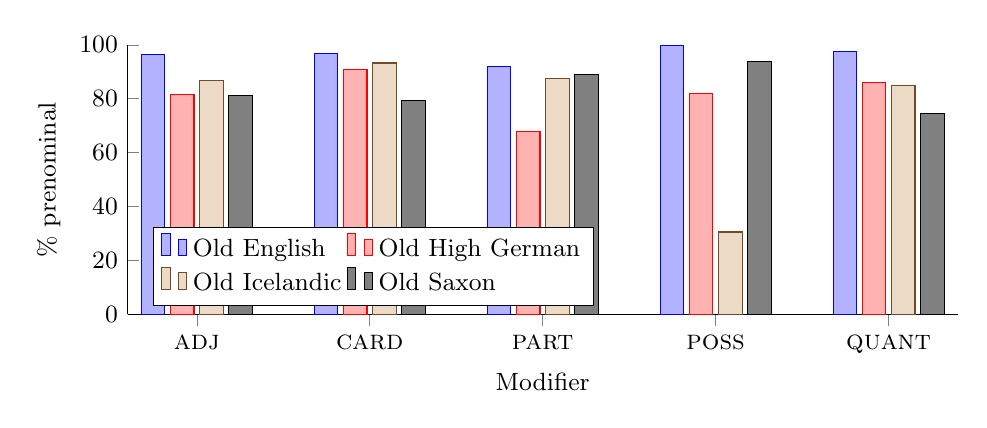
\begin{tikzpicture}
\begin{axis}
	[axis lines*=left,
	bar width=.3cm,
	height  = 5cm,
	font=\small,
	legend pos=south west,
	legend cell align=left,
	legend columns=2,
	symbolic x coords={adj,card,part,poss,quant},
	xticklabel style = {font=\scshape},
	width  = \textwidth,
	xtick=data,
	x tick label style={},
	xlabel=Modifier,
	ybar,
	ylabel=\% prenominal,
	ymin=0,
	ymax=100
	]
	\addplot coordinates
	  { 
	  	(adj,96.6)
	  	(card,96.7)
	  	(part,92.1)
	  	(poss,99.7)
	  	(quant,97.6) 
	  };
	\addlegendentry{Old English}
	\addplot coordinates
	  { 
		(adj,81.7)
		(card,90.9)
		(part,67.7)
		(poss,82.0)
		(quant,86.1) 
	  };
    \addlegendentry{Old High German}
	\addplot coordinates
	  { 
		(adj,86.9)
		(card,93.3)
		(part,87.5)
		(poss,30.5)
		(quant,84.8) 
	  };
	\addlegendentry{Old Icelandic}
	\addplot coordinates
	  { 
		(adj,81.3)
		(card,79.4)
		(part,88.9)
		(poss,93.7)
		(quant,74.4) 
	  };
	\addlegendentry{Old Saxon}
\end{axis}
\end{tikzpicture}

\caption{Modifier–noun order in Old English, Old High German, Old Icelandic, and Old Saxon}
\label{figone}
\end{figure}

\begin{table}[H]
\caption{Modifier–noun order in Old English, Old High German, Old Icelandic, and Old Saxon}
\label{taboverview}
 \begin{tabularx}{\textwidth}{l Yr Yr Yr Yr }
  \lsptoprule
  & \multicolumn{2}{c}{OE} & \multicolumn{2}{c}{OHG} & \multicolumn{2}{c}{OI} & \multicolumn{2}{c}{OS}\\
  \cmidrule(lr){2-3}\cmidrule(lr){4-5}\cmidrule(lr){6-7}\cmidrule(lr){8-9}
           & n        & \%     & n     & \%   & n     & \%   & n      & \%\\
  \midrule
  ADJ--N   & 40\,957   & 96.6   & 3\,097 & 81.7 & 3\,529  & 86.9 & 1\,335 & 81.3\\
  N--ADJ   & 1\,454    & 3.4    & 694   & 18.3 & 532    & 13.1 & 307   & 18.7\\
  CARD--N  & 8\,075    & 96.7   & 662   & 90.9 & 616    & 93.3 & 108   & 79.4\\
  N--CARD  & 278      & 3.3    & 66    & 9.1  & 44     & 6.7  & 28    & 20.6\\
  PART--N  & 2\,190    & 92.1   & 176   & 67.7 & 77     & 87.5 & 64    & 88.9\\
  N--PART  & 189      & 7.9    & 84    & 32.3 & 11     & 12.5 & 8     & 11.1\\
  POSS--N  & 29\,647   & 99.7   & 3\,528 & 82.0 & 1\,339  & 30.5 & 1\,403 & 93.7\\
  N--POSS  & 78       & 0.3    & 774   & 18.0 & 3\,057  & 69.5 & 94    & 6.3 \\
  QUANT--N & 18\,179   & 97.6   & 1\,350 & 86.1 & 1\,742  & 84.8 & 261   & 74.4\\
  N--QUANT & 442      & 2.4    & 218   & 13.9 & 312    & 15.2 & 90    & 25.6\\
  \midrule
  MOD--N   & 99\,048   & 97.6   & 8\,813 & 82.8 & 7\,303  & 64.9 & 3\,171 & 85.7 \\
  N--MOD   & 2\,441    & 2.4    & 1\,836 & 17.2 & 3\,956  & 35.1 & 527   & 14.3 \\
  \lspbottomrule
 \end{tabularx}
\end{table}
\pagebreak

In Sections \ref{ssectANNA}--\ref{ssectQNNQ} we give examples of the different patterns presented in \tabref{taboverview}. We exemplify each \isi{pattern} from one or two languages, but all the languages show all the patterns, though to different extents. 

\subsection{Adjective–Noun, Noun–Adjective}\label{ssectANNA}

This group contains adjectives that either stand alone before or after the \isi{noun} or occur together with other modifiers. 


% \noindent Old \ili{English}
% \ea\label{OEAN}
% ADJ--N\\
% \gll Se \textbf{frumsceapena} \textit{mann} Adam næs gestryned ne acenned\\
% \DEF.\NOM.\SG{} first.created.\NOM.\SG.\WK{} man.\NOM.\SG{} Adam.\NOM.\SG{} not.was begotten not born\\
% \glt ‘The first man, Adam, was neither begotten nor born.’ (cocathom2,+ACHom\_II,\_1:4.59.41)
% \z
%
% \ea\label{OENA}
% N--ADJ\\
% \gll Se þridda het Heanric, þam se fæder becwæð \textit{gersuman} \textbf{unateallendlice}\\
% 	\DEF{} third was.called Henry \DEF.\DAT.\SG{} \DEF{} father bequeathed treasure.\ACC.\PL{} innumerable.\ACC.\PL.\STR{}\\
% \glt‘The third was called Henry, to whom the father left innumerable treasures.' (cochronE,ChronE\_[Plummer]:1086.59.2889)
% \z

\begin{exe}
\ex\label{OEAN}
Old \ili{English}
\ea ADJ--N\\
\gll Se \textbf{frumsceapena} \textit{mann} Adam næs gestryned ne acenned\\
\DEF.\NOM.\SG{} first.created.\NOM.\SG.\WK{} man.\NOM.\SG{} Adam.\NOM.\SG{} not.was begotten not born\\
\glt ‘The first man, Adam, was neither begotten nor born.’ (cocathom2,+ACHom\_II,\_1:4.59.41)
\ex\label{OENA}
N--ADJ\\
\gll Se þridda het Heanric, þam se fæder becwæð \textit{gersuman} \textbf{unateallendlice}\\
	\DEF{} third was.called Henry \DEF.\DAT.\SG{} \DEF{} father bequeathed treasure.\ACC.\PL{} innumerable.\ACC.\PL.\STR{}\\
\glt‘The third was called Henry, to whom the father left innumerable treasures.' (cochronE,ChronE\_[Plummer]:1086.59.2889)
\z
\end{exe}

The constituent \textit{uteweardum} in (\ref{OENA2}) represents a special category of modifiers named “positional predicates”, discussed in \textcitetv{chapters/10PosPredOG}. Positional predicates agree in case, gender and number with the head \isi{noun}, but semantically they resemble adverbs/adverbials. These behave differently from other adjectives; one prominent feature is that they occur postnominally. 

\ea\label{OENA2}
N--ADJ\\
\gll Þa gefengon hi þara ðreora scypu twa æt þam \textit{muþan} \textbf{uteweardum}\\
	then captured they \DEF.\GEN{} three.\textsc{gen} ships.\textsc{acc} two.\textsc{acc} at \DEF.\DAT.\SG{} mouth.\DAT.\SG{} 	outside.\DAT.\SG.\STR{}\\
\glt ‘Then they captured two of the three ships outside the river mouth.’ (cochronC,ChronC\_[Rositzke]:897.26.991)
\z



The two patterns (ADJ–N, N–ADJ) can also be found within a complex \isi{noun} phrase, e.g. (\ref{OIANNA}). 


\ea\label{OIANNA}
\noindent \ili{Old Icelandic}\medskip\\
ADJ--N and N--ADJ\\
\gll {af því að} hann var \textbf{fésnauður} \textit{maður} en \textit{drengur} \textbf{góður} og karlmaður í skapi\\
because he was poor.\NOM.\SG.\STR{} man.\NOM.\SG{} but fellow.\NOM.\SG{} good.\NOM.\SG.\STR{} and man.of.valour in mind\\
\glt ‘because he was a poor man but a good fellow and a man of valorous mind’ (1210.JARTEIN.REL-SAG,.29)
\z

\subsection{Cardinal numeral–Noun, Noun–Cardinal numeral}\label{ssectCaNNCa}

Here we include cardinal numerals in pre- or \isi{postnominal} position. The numerals may occur together with other elements.


\ea\label{OSCardN}
\ili{Old Saxon}\\
\ea CARD--N\\
\gll Giuuet im thuo umbi \textbf{thria} \textit{naht} aftar thiu […] an Galilealand thesaro thiedo drohtin\\
went he.\DAT{} then about three.\ACC.\PL{} night.\ACC.\PL{} after \DEM{} {} to Galilee \DEM.\GEN.\SG/\PL{} people.\GEN.\SG/\PL{} lord.\NOM.\SG{}\\
\glt ‘Then the lord of this people went to Galilee, about three nights after that.’ (HeliandC.1027.1994-1996)

\ex\label{OSNCard}
N--CARD\\
\gll endi hiet sia nahor gangan, Andrease endi Petruse erist sane, \textit{gibruother} \textbf{tuena}\\
and called they.\ACC{} nearer go Andrew and Peter first soon brother\ACC.\PL{} two.\ACC.\PL{}\\
\glt ‘and called them to come closer, Andrew and Peter at first, two brothers’ (HeliandC.686.1255-1258)
\z
\ex\label{OHGCardN}
\noindent Old High \ili{German}\\
\ea CARD--N\\
\gll Huuer uuac \textbf{dhrim} \textit{fingrum} allan aerdhuuasun?\\
who weighed three.\DAT.\PL{} finger.\DAT.\PL{} all earth\\
\glt ‘Who weighed the whole earth with three fingers?’\\
(Isidor\_1.1 > I\_DeFide\_4 (edition 805--815))
\ex\label{OHGNCard}
N--CARD\\
\gll Wir duemes tház […] mit unsen \textit{fíngoron} \textbf{zuein}\\
we do \DEM{} {} with our finger.\DAT.\PL{} two.\DAT.\PL{}\\
\glt ‘We do this […] with our two fingers.’\\
(Otfrid\_1.1 > O\_Otfr.Ev.5.2 (edition 68--78))
\z
\z

\subsection{Possessive–Noun, Noun–Possessive}\label{ssectPosNNPos}

The YCOE \isi{corpus} (Old \ili{English}) and the HeliPaD \isi{corpus} (\ili{Old Saxon}) treat possessive pronouns differently from the IcePaHC \isi{corpus} (\ili{Old Icelandic}), but crucially all corpora mark them as distinct from non-possessive pronouns, so we were able to get comparable datasets across the corpora, via corpus-specific searches. The point to take home for Old \ili{English} is that possessives are extremely rare postnominally. \ili{Old Icelandic}, on the other hand, is different from the other varieties in favouring the order \isi{noun}–possessive, as shown in \tabref{taboverview}.\largerpage


\ea\label{OIPossN}
\noindent \ili{Old Icelandic}
\ea
POSS--N\\
\gll En þeir feðgar ríða heim með \textbf{sína} \textit{menn}\\
	and they {father and son} ride home with their.\REFL.\ACC.\PL{} man.\ACC.\PL{}\\
\glt	‘And father and son ride home with their men.’
(1350.FINNBOGI.NAR-SAG,663.2204)
\ex\label{OINPoss}
N--POSS\\
\gll og hann skal sitja fyr \textit{ádrykkju} \textbf{minni} {í kveld}\\
	and he shall sit before drinking.\DAT.\SG{} my.\DAT.\SG{} tonight\\
\glt `and he shall sit as my drinking-mate tonight’ (1275.MORKIN.NAR-HIS,.1574)
\z
\ex\label{OSPossN}
\noindent \ili{Old Saxon}
\ea POSS--N\\
\gll diuridon \textbf{usan} \textit{drohtin}\\
	glorified our.\ACC.\SG{} lord.\ACC.\SG{}\\
\glt ‘(They) glorified our lord.’ (HeliandC.32.83)
\ex\label{OSNPoss}
N--POSS\\
\gll dopta allan dag druhtfolc mikil, uuerod an uuatere […] \textit{handon} \textbf{sinon}\\
baptized all day people great people in water {} hand.\DAT.\PL{} his.\DAT.\PL{}\\
\glt ‘(He) baptized the great multitude in water all day with his hands.’ (HeliandC.533.978-981)
\z
\z
\pagebreak
\subsection{Participle–Noun, Noun–Participle}\label{ssectPartNNPart}
This category comprises both present and past participles, with or without \isi{agreement} marking.\footnote{Postnominal
  participles are often small clauses rather than \isi{attributive} adjectives, as in (\ref{smallclause}) from Old \ili{English}.
  \ea\label{smallclause}
  \gll Nu ic geseo minne \textit{geleafan} \textbf{blowende} and mine \textit{sawle} \textbf{anlyht} and þysne \textit{dracan} \textbf{acwealdne} licgean \\
          now I see my.\ACC.\SG{} faith.\ACC.\SG{} flourishing.\ACC.\SG.\STR{} and my.\ACC.\SG{} soul.\ACC.\SG{} illuminated.\ACC.\SG.\STR{} and \DEM.\ACC.\SG{} dragon.\ACC.\SG{} killed.\ACC.\SG.\STR{} lie\\
  \glt ‘Now I see my faith flourishing and my soul illuminated and this dragon lie killed.’ (comargaT,LS\_16\_[MargaretCot.Tib.\_A.iii]:13.10.152)
  \z}


\ea\label{OHGPartN}
\noindent Old High \ili{German}
\ea
PART--N\\
\gll ih bisueru thih bi themo \textbf{lebenten} \textit{gote}\\
I beseech you for \DEF.\DAT.\SG{} living.\DAT.\SG.\WK{} god.\DAT.\SG{}\\
 \glt ‘I beseech you for the sake of the living God.’\\ (Tatian\_1.1 > T\_Tat190 (edition 9-19))
\ex\label{OHGNPart}
N--PART\\
\gll Galih ist himilo rihhi \textit{gaberge} \textbf{gabor}(\textbf{ga})\textbf{nemo} in acchre\\
similar is heaven’s kingdom treasure.\DAT.\SG{} hidden.\DAT.\SG.\STR{} in field\\
\glt ‘The kingdom of heaven is like a sacred store of wealth in a field.’ (Monsee\_1.1 > MF\_1\_M.X (edition 106--116))
\z
\ex\label{OEPartN}
\noindent Old \ili{English}
\ea PART--N\\
\ea
\gll and of heora muðe and nosþyrlum stod \textbf{stincende} \textit{steam}\\
and of her mouth and nostrils stood stinking.\NOM.\SG.\STR{} steam.\NOM.\SG{}\\
\glt ‘and her mouth and nostrils emitted stinking vapour’ (cocathom2,+ACHom\_II,\_23:200.49.4451)
\ex\label{OEPartN2}
\gll \& \textbf{gebigedum} \textit{cneowum} gebæd for ðam folce\\
	and bent.\DAT.\PL.\STR{} knee.\DAT.\PL{} prayed for \DEF{} people\\
\glt ‘and prayed for the people with bent knees’ (cotempo,+ATemp:11.5.354)
\z

\ex\label{OENPart}
N--PART\\
\gll se nama tacnaþ þone sige þe \textit{Drihten} \textbf{gesigefæsted} wiþstod deofle\\
\DEF{} name marks \DEF{} victory that Lord.\NOM.\SG{} triumphant.\NOM.\SG.\STR{} withstood devil\\
\glt ‘the name marks the victory in which the triumphant Lord withstood the devil’ (coblick,HomS\_21\_[BlHom\_6]:67.18.815)
\z
\z

\subsection{Quantifier–Noun, Noun–Quantifier}\label{ssectQNNQ}
Here we searched for any \isi{quantifier}.


\ea\label{OOIQN}
\ili{Old Icelandic}
\ea QUANT--N\\
\gll og tók nú Knútur við Hollsetulandi og \textbf{öllu} því \textit{ríki} er átt hafði Haraldur jarl\\
and took now Knútur with Holstein and all.\DAT.\SG{} \DEM.\DAT.\SG{}
kingdom.\DAT.\SG{} which possessed had Haraldur earl\\
\glt ‘and now Knútur accepted Holstein and all that kingdom which Earl Haraldur had possessed’ (1260.JOMSVIKINGAR.NAR-SAG,.309)
\ex\label{OINQ}
N--QUANT\\
\gll Það er mælt um \textit{sakir} þær \textbf{allar} sem hér eru taldar\\
	it is spoken about case.\ACC.\PL{} \DEM.\ACC.\PL{} all.\ACC.\PL{} which here are told\\
\glt ‘It is spoken about all those cases which are told here.’
(1270.GRAGAS.LAW-LAW,.334)
\z
\z

\ea\label{OSQN}
\ili{Old Saxon}\\
\ea QUANT--N\\
\gll Thar hie sittean fand Andrease endi Petruse bi them ahastrome, \textbf{bethia} thia \textit{gibruođer}\\
there he sit found Andrew and Peter by \DEF{} water.stream both.\ACC.\PL{} \DEF.\ACC.\PL{} brother.\ACC.\PL{}\\
\glt ‘There he found Andrew and Peter sitting by the river, both the brothers.’ (HeliandC.630.1152-1156)
\pagebreak\ex\label{OSNQ}
N--QUANT\\
\gll Uuerthe thin uuilleo oƀar thesa \textit{uuerold} \textbf{alla}\\
	become.\SBJV{} your will over \DEM.\ACC.\SG{} world.\ACC.\SG{} all.\ACC.\SG{}\\
\glt ‘Your will be done over all this world.’ (HeliandC.853.1604-1606)
\z
\z


\section{Discussion: Specific factors in the different languages}\label{sectdisc}\largerpage

In this section we examine whether there are specific factors in the different languages that influence the element order. We specifically consider the influence of text types, different types of possessive modifiers, \isi{weight}, individual lexical items, \isi{lexicalized} patterns, and whether the adjectives flank the head \isi{noun}. We have not considered all these factors for each language, but rather picked out factors to investigate more closely on the basis of \tabref{taboverview}. We assume that these factors could be at play in all the languages, but selected those languages for which these factors were most clearly influential. 

\subsection{Old High German texts and genres}\label{ssectOHGtextgenres}
As outlined in Section \ref{sectdata}, the Old High \ili{German} \isi{corpus} consists of poems and vernacular translations of \ili{Latin} sources, both making it methodologically unjustified to simply assume that the attested \isi{word order} patterns represent genuine Old High \ili{German} grammar. Applied to the question at issue, this means that the \isi{variation} in the order of nouns and modifiers illustrated in the examples above may be the result of metrical considerations or of non-native loan \isi{syntax}, rather than of independent, language-internal factors. As the degree of dependence of the vernacular writings on the \isi{word order} of the \ili{Latin} original differs among the individual translations, the method of comparing the source \isi{syntax} and its representation in the translations has become a leading principle in assessing evidence for native Old High \ili{German} grammar (\cite{DittmerDittmer98}; \cite{Donhauser98}; \cite{Fleischer06}; \cite{Fleischeretal08}). 
	
 To test how factors such as \isi{genre} and loan \isi{syntax} affect the \isi{word order} in \isi{noun} phrases in Old High \ili{German}, the number of pre- and \isi{postnominal} modifiers was retrieved and compared for individual texts as representatives of the following three text types:

 \begin{enumerate}[label=(\roman*)]
     \item poetry, represented by Otfrid’s \textit{Gospel Book} and the poetic records included in Steinmeyer’s \citeyearpar{vonSteinmeyer16} collection of Minor Old High \ili{German} documents;
     \item interlinear translations such as the \textit{Benediktinerregel} and \textit{Murbacher Hymnen} as representatives of the strict form-by-form and word-by-word type of translations;
     \item non-interlinear translations such as the copy of Isidorus’s treaty \textit{De Fide}, the texts comprised in the manuscript collection called the \textit{Monsee Fragments} and the translation of Tatian’s \textit{Gospel Harmony} into Old High \ili{German}.
 \end{enumerate}

The frequencies of adnominal modifiers of the various types, surfacing in pre- and \isi{postnominal} position, were retrieved for these three types of texts individually from the ReA \isi{corpus}. They are provided in \tabref{tabOHGtext} and visualized in \figref{figtwo}.

\begin{table}
\caption{Pre- and postnominal modifiers in poetry, interlinear translations and non-interlinear translations in Old High German}
\label{tabOHGtext}
%  \begin{tabularx}{\textwidth}{l Y@{~~}r Y@{~~}r Y@{~~}r Y@{~~}r Y@{~~}r}
%   \lsptoprule
% & \multicolumn{2}{c}{ADJ} & \multicolumn{2}{c}{CARD} & \multicolumn{2}{c}{POSS} & \multicolumn{2}{c}{PART} & \multicolumn{2}{c}{QUANT}\\
%   \cmidrule(lr){2-3}\cmidrule(lr){4-5}\cmidrule(lr){6-7}\cmidrule(lr){8-9}\cmidrule(lr){10-11}
% & \rotatebox{90}{ADJ--N} & \rotatebox{90}{N--ADJ} & \rotatebox{90}{CARD--N} & \rotatebox{90}{N--CARD} & \rotatebox{90}{POSS--N} & \rotatebox{90}{N--POSS} & \rotatebox{90}{PART--N} & \rotatebox{90}{N--PART} & \rotatebox{90}{QUANT--N} & \rotatebox{90}{N--QUANT}\\
% \midrule
% \multicolumn{10}{l}{\textbf{Poetry}}\\
% \midrule
% n & 973 & 276 & 105 & 17 & 1,232 & 370 & 23 & 11 & 372 & 181\\
% \% & 77.9 & 22.1 & 86.1 & 13.9 & 76.9 & 23.1 & 67.6 & 32.4 & 67.3 & 32.7\\
%
% \tablevspace
% \multicolumn{10}{l}{\textbf{Interlinear translations}}\\
% \midrule
% n & 403 & 139 & 97 & 7 & 62 & 157 & 51 & 31 & 131 & 7\\
% \% & 74.4 & 25.6 & 93.3 & 6.7 & 28.3 & 71.7 & 62.2 & 37.8 & 94.9 & 5.1\\
%  \tablevspace
% \multicolumn{10}{l}{\textbf{Non-interlinear translations}}\\
% \midrule
% n & 634 & 79 & 281 & 4 & 1,591 & 15 & 30 & 22 & 442 & 13 \\
% \% & 88.9 & 11.1 & 98.6 & 1.4 & 99.1 & 0.9 & 57.7 & 42.3 & 97.1	& 2.9 \\
%  \lspbottomrule
%  \end{tabularx}
\begin{tabular}{ll rr rr rr}
\lsptoprule
       &      &     &     & \multicolumn{2}{c}{Interlinear}&\multicolumn{2}{c}{Non-interlinear}\\
       &      & \multicolumn{2}{c}{Poetry}  &\multicolumn{2}{c}{translations} & \multicolumn{2}{c}{translations}\\
       \cmidrule(lr){3-4}\cmidrule(lr){5-6}\cmidrule(lr){7-8}
       & & n & \%& n & \%& n & \%\\
   \midrule
   ADJ & ADJ--N   & 973   & 77.3 & 403 & 74.4 & 634  & 88.9\\
       & N--ADJ   & 276   & 22.1 & 139 & 25.6 & 79   & 11.1\\
   CARD & CARD--N & 105   & 86.1 & 97  & 93.3 & 281  & 98.6 \\
        & N--CARD & 17    & 13.9 & 7   & 6.7  & 4    & 1.4  \\
   PART & PART--N & 23    & 67.6 & 51  & 62.2 & 30   & 57.7 \\
        & N--PART & 11    & 32.4 & 31  & 37.8 & 22   & 42.3 \\
   POSS & POSS--N & 1\,232  & 76.9 & 62  & 28.3 & 1\,591 & 99.1 \\
        & N--POSS & 370   & 23.1 & 157 & 71.7 & 15   & 0.9 \\
   QUANT & QUANT--N & 372 & 67.3 & 131 & 94.9 & 442  & 97.1 \\
         & N--QUANT & 181 & 32.7 & 7   & 5.1  & 13   & 2.9\\
\lspbottomrule
\end{tabular}
\end{table}

\begin{figure}
% \includegraphics[height=.35\textheight]{figures/ohg-graph.png}
\pgfplotsset{/pgfplots/bar cycle list/.style={/pgfplots/cycle list name={langsci-RdYlBl-4}}}
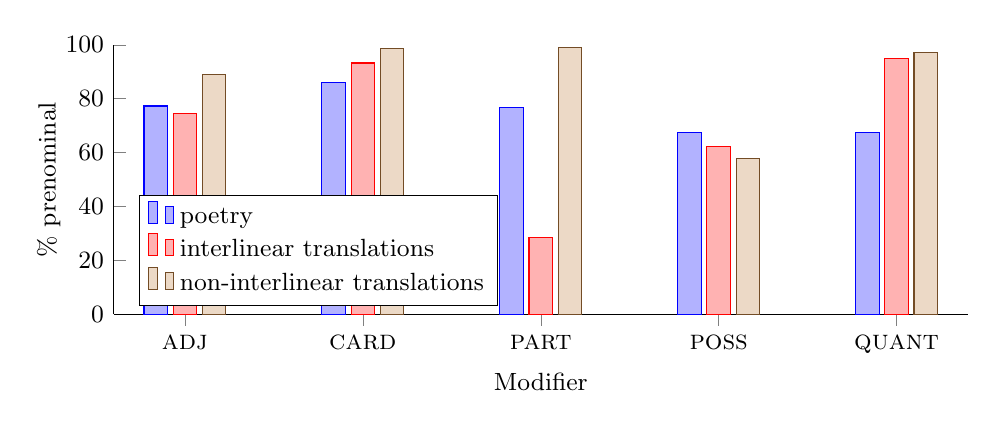
\begin{tikzpicture}
\begin{axis}
	[axis lines*=left,
	bar width=.3cm,
	height  = 5cm,
	font=\small,
	legend pos=south west,
	legend cell align=left,
	legend columns=1,
	symbolic x coords={adj,card,part,poss,quant},
	xticklabel style = {font=\scshape},
	width  = 1.025\textwidth,
	xtick=data,
	x tick label style={},
	xlabel=Modifier,
	ybar,
	ylabel=\% prenominal,
	ylabel near ticks, 
	ylabel shift={-5pt},
	ymin=0,
	ymax=100
	]
    \addplot coordinates
	  { 
		(adj,77.3)
		(card,86.1)
		(part,76.9)
		(poss,67.6)
		(quant,67.3) 
	  };
    \addlegendentry{poetry}
	\addplot coordinates
	  { 
	  	(adj,74.4)
	  	(card,93.3)
	  	(part,28.3)
	  	(poss,62.2)
	  	(quant,94.9) 
	  };
	\addlegendentry{interlinear translations}
	\addplot coordinates
	  { 
		(adj,88.9)
		(card,98.6)
		(part,99.1)
		(poss,57.7)
		(quant,97.1) 
	  };
	\addlegendentry{non-interlinear translations}
\end{axis}
\end{tikzpicture}
\caption{Pre- and postnominal modifiers in poetry, interlinear translations and non-interlinear translations in Old High German}
\label{figtwo}
\end{figure}

The numbers in \tabref{tabOHGtext} give rise to some important generalizations. First, they confirm the observation that could be inferred from \tabref{taboverview}, namely that participles used as modifiers have a unique status among modifiers in that they tend to follow their head nouns more independently of the text type, i.e. independently of factors such as rhyme or loan \isi{syntax}. Note that participles score even higher in \isi{postnominal} position in non-interlinear translations than in poetry and texts with a high degree of loan \isi{syntax}, which suggests that this is a genuine property that modifying participle phrases share with clausal modifiers, e.g. \isi{attributive} relative clauses, in Old High \ili{German}. 

Apart from participles, all remaining modifying categories display lower frequencies of \isi{postnominal} position in non-interlinear translations than in the remaining two types of texts. For cardinal numbers, possessives and quantifiers, the percentage of \isi{postnominal} modifiers in non-interlinear translations is almost negligible, below 3\% of all attested cases. Adjectives surface after the \isi{noun} in non-interlinear translation more often than with cardinal numerals, possessive and quantifiers, i.e. in 11.1\% of the cases, but this frequency is lower that the overall one in \tabref{taboverview}, which is 18.3\%. 

A closer look at the Old High \ili{German} patterns in non-interlinear translations and their relation to the \ili{Latin} sources reveals that the proportion of independently produced, and thus native, \isi{postnominal} categories is even lower than the numbers in \tabref{tabOHGtext} suggest. Consider the numbers in \tabref{tabOHGILL}.

\begin{table}
\caption{Latin influence on postnominal modifiers in non-interlinear translations in Old High German (participles are excluded)}
\label{tabOHGILL}
 \begin{tabular}{l@{}rrrr}
  \lsptoprule
  & Equal to Latin  & Different from Latin & {Misparsings} & {Total} \\
  \midrule
  N--ADJ & 66 & 4 & 9 & 79\\
  N--CARD & 3 & 1 & 0 & 4\\
  N--POSS & 14 & 0 & 1 & 15\\
  N--QUANT & 11 & 2 & 0 & 13\\
  \lspbottomrule
 \end{tabular}
\end{table}

\tabref{tabOHGILL} shows that the frequency of \isi{postnominal} modifiers not influenced by \ili{Latin} is extremely low in non-interlinear translations. For example, possessives are never attested in \isi{postnominal} position if there is no corresponding \ili{Latin} sentence displaying this \isi{pattern}. With cardinals, there is a single example (\ref{OHGNCard2}) in which the Old High \ili{German} text contains a \isi{postnominal} cardinal \isi{numeral} independently of the \ili{Latin} original. Note that the corresponding \ili{Latin} \isi{pattern} involves a single cardinal \textit{duos} ‘two.\textsc{acc.pl}’ selecting the prepositional phrase \textit{de discipulis suis} ‘of his disciples’ as a complement. In other words, not only does the Old High \ili{German} translation change the order of the cardinal and the reflexive possessive relative to the \isi{noun}, but also the structure within the object phrase. 

\ea\label{OHGNCard2}
\gll gihalota / sine \textit{iungiron} \textbf{zuene}\\
called {}  his disciple.\ACC.\PL{} two.\ACC.\PL{}\\
\glt ‘(He) called his two disciples.’ (Tatian\_1.1 > T\_Tat64 (edition 10--20))
\glt Lat. convocans / duos de discipulis suis 
\z

Regarding adjectives, the picture is similar. The comparison between the \ili{Latin} original and the vernacular translation reveals that in only 4 of 79 examples does the scribe opt for a \isi{postnominal} placement of the respective modifier independently of its position in the source text. Three of these examples, however, are less conclusive. One is (\ref{OHGfolle}), where the \isi{adjective} \textit{folle} forms the extended phrase ‘full of hate’, which is used as an apposition postposed after the head \isi{noun}. The second one is (\ref{OHGal}), which involves the \isi{quantifier} \textit{al} annotated as an \isi{adjective}, probably because it translates the \isi{prenominal} \ili{Latin} \isi{adjective} \textit{universus}. The third one, given in (\ref{OHGdodemu}), is special in that it involves a very infrequent Old High \ili{German} \isi{pattern} used to translate the absolute constructions of the \ili{Latin} original. One valid example with a \isi{postnominal} \isi{adjective} remains, given in (\ref{OHGdhrifaldan}). It is found in the oldest one of the three translations taken into consideration, suggesting that the independent \isi{postnominal} use of adjectives is likely a non-productive \isi{pattern} only present in the earliest phase of the Old High \ili{German} attestation.

\ea\label{OHGfolle}
\gll iudea \textit{liuti} \textbf{nides} \textbf{folle}\\
Jewish people.\NOM.\PL{} hate.\GEN.\SG{} full.\NOM.\PL.\STR{}\\
\glt ‘the Jewish people, full of hate’ \\
(Monsee\_1.1 > MF\_2\_VG.XXXI (edition 186--206))
\glt Lat. iudei repleti sunt zelo at inuidia 	
\z
						
\ea\label{OHGal}
\gll Tho antlingita thaz \textit{folc} \textbf{al}\\
	then replied \DEF.\NOM.\SG{} crowd.\NOM.\SG{} all.\NOM.\SG{}\\
\glt ‘Then the whole crowd replied.’ (Tatian\_1.1 > T\_Tat199 (edition 250--260))
\glt Lat. Et respondens universus populus	
\z
							
\ea\label{OHGdodemu}
\gll after \textit{moysise} \textbf{dodemu}\\
after Moses.\DAT.\SG{} dead.\DAT.\SG.\STR{}\\
\glt ‘after the death of Moses’ (Isidor\_1.1 > I\_DeFide\_6 (edition 70--80))
\glt Lat. defuncto moyse
\z
							
\ea\label{OHGdhrifaldan}
\gll dhazs dher forasago auh dhen selbun \textit{druhtin} \textbf{dhrifaldan} in sinem heidim araughida\\
that \DEF{} prophet also \DEF{} same Lord.\ACC.\SG{} threefold.\ACC.\SG.\STR{} in his shape showed\\
\glt ‘that the prophet referred to the same threefold Lord in his manifestations’ (Isidor\_1.1 > I\_DeFide\_4 (edition 929--939))
\glt Lat. Quem ut trinum in personis ostenderet
\z

Let us look at the quantifiers. As the numbers in \tabref{tabOHGILL} suggest, in 11 out of 13 examples, the \isi{postnominal} \isi{quantifier} in Old High \ili{German} is explainable as a syntactic loan, given that the \ili{Latin} original also displays a \isi{postnominal} \isi{quantifier}. In two examples, given in (\ref{OHGsibun}) and (\ref{OHGmanagen}), the \isi{quantifier} is \isi{prenominal} in the \ili{Latin} original but \isi{postnominal} in the translation. The fact that there are two modifying categories present in the examples will be discussed in detail in Section \ref{ssectFlanked} below.

\ea\label{OHGsibun}
\gll sibun \textit{geista} \textbf{andere} mit imo\\
seven spirit.\ACC.\PL{} other.\ACC.\PL.\STR{} with him\\
\glt ‘seven other spirits with him’ (Tatian\_1.1 > T\_Tat57 (edition 194--204))
\glt Lat. septem alios spiritus secum
\z						

\ea\label{OHGmanagen}
\gll Inti sulihhen \textit{ratissun} \textbf{managen}\\
	and such.\DAT.\PL.\STR{} parable.\DAT.\PL{} many.\DAT.\PL.\STR{}\\
\glt ‘and with many such parables’ (Tatian\_1.1 > T\_Tat74 (edition 38--48))
\glt Lat. et talibus multis parabolis
\z							

\subsection{Possessive modifiers in Old Saxon and Old Icelandic}\label{ssectPossOSOI}

\begin{sloppypar}
In \ili{Old Saxon}, whether a possessive modifier can be \isi{postnominal} or not is determined by person and number. Specifically, the indeclinable modifiers \textit{is} (\POSS.3\SG.\MASC/\N) and \textit{iro} (\POSS.3\SG.\FEM, \POSS.3\PL), which are simply the \isi{genitive} forms of the corresponding pronouns, are always \isi{prenominal} (814/814 examples in the HeliPaD). By \isi{contrast}, the other possessives \textit{min} (\POSS.1\SG), \textit{unka} (\POSS.1\DU), \textit{usa} (\POSS.1\PL), \textit{thin} (\POSS.2\SG), \textit{inka} (\POSS.2\SG), \textit{iuwa} (\POSS.2\PL), and \textit{sin} (\POSS.\REFL) are all declined as adjectives, and these forms may be either \isi{prenominal} (507/589; 86\%) or \isi{postnominal} (82/589; 14\%).
\end{sloppypar}

\ili{Old Icelandic} pronominal possessors inflect like strong adjectives and are often considered to belong to the same class (\cite[20]{Heltoft10}; \cite{Barnes08}). However, with respect to order they \isi{pattern} radically differently. As the data in \tabref{tabOIAPoss} (taken from \tabref{taboverview}, but presented separately for clarity) show, while adjectives are predominantly \isi{prenominal}, the predominant \isi{pattern} for pronominal possessors is \isi{postnominal}. In this respect, \ili{Old Icelandic} pronominal possessors may show similar positional behaviour to pronominal possessors in \ili{Gothic} (\cite[see][213]{ratkus2011}), but diverge strikingly from parallel elements in Old \ili{English} and \ili{Old Saxon}.

\begin{table}
\caption{Position of adjectives and pronominal possessors in Old Icelandic (1150–1350)}
\label{tabOIAPoss}
\begin{tabular}{l rr rr}
\lsptoprule
& \multicolumn{2}{c}{Prenominal} & \multicolumn{2}{c}{Postnominal}\\\cmidrule(lr){2-3}\cmidrule(lr){4-5}
& $n$ & \% & $n$ & \%\\\midrule
ADJ & 3\,529 & 86.9 & 532 & 13.1\\
POSS & 1\,339 & 30.5 & 3\,057 & 69.5\\
\lspbottomrule
\end{tabular}
\end{table}

Examples of \isi{prenominal} and \isi{postnominal} pronominal posessors are shown in (\ref{OIprenPoss}) and (\ref{OIpostPoss}), respectively. 

\ea\label{OIprenPoss}
\gll Nú fara \textbf{sína} \textit{leið} hvorir\\
now goes his.\REFL.\ACC.\SG{} way.\ACC.\SG{} each\\
\glt ‘Now each one goes his own way.’ (1310.GRETTIR.NAR-SAG,.1542)
\ex\label{OIpostPoss}
\gll Stigu þeir Svarthöfði á bak og fóru \textit{leið} \textbf{sína}\\
	stepped they Svarthöfði onto back and went way.\ACC.\SG{} their.\REFL.\ACC.\SG{}\\
\glt ‘They and Svarthöfði mounted the horses and went on their way.’ (1250.STURLUNGA.NAR-SAG,.401.492-493)
\z

\citet[19--20]{Borjarsetal16} argue that the \isi{prenominal} position for pronominal possessors may be associated with information-structural properties such as \isi{contrast} or \isi{emphasis}. The natural use of ‘own’ in the idiomatic translation of (\ref{OIprenPoss}) may be taken to support this claim. As we saw in Section \ref{ssectprev}, the assumption in the literature is that the \isi{postnominal} position is canonical and the \isi{prenominal} position emphatic or otherwise marked also for \isi{adjective} phrases, but the data in Tables \ref{taboverview} and \ref{tabOIAPoss} make this an unlikely scenario.

\subsection{Weight matters: Old English and Old Icelandic}\label{ssectweight}

It has been shown that \isi{weight} matters when it comes to element order at clausal level (see e.g. \cite{TaylorPintzuk2012} for Old \ili{English}). And indeed, the Old \ili{English} data indicate that this is the case with respect to \isi{noun} phrase constituents as well (see also \cite{Grabski17}).

In \tabref{tabOEweight}, “simple AP" refers to \isi{adjective} phrases consisting of just one \isi{adjective} and “complex AP" refers to a phrase where the \isi{adjective} is modified or combined with a complement. 

\begin{table}
\caption{Position of simple adjective phrases and complex adjective phrases in Old English (excluding flanked adjectives)}
\label{tabOEweight}

 \begin{tabular}{l rrrr}
  \lsptoprule
  & \multicolumn{2}{c}{Prenominal} & \multicolumn{2}{c}{Postnominal}\\\cmidrule(lr){2-3}\cmidrule(lr){4-5}
  & $n$ & \% & $n$ & \%\\
  \midrule
 Simple AP & 40\,957 & 96.6 & 1\,454 & 3.4\\
 Complex AP & 950 & 72.1 & 367 & 27.9\\
 \lspbottomrule
 \end{tabular}
\end{table}

When the \isi{adjective} phrase consists of one \isi{adjective} (simple AP), it overwhelmingly occurs prenominally. If the AP is complex, it still occurs prenominally in the majority of cases, but about a quarter of the cases occur postnominally. Example (\ref{OEprenComp}) shows a \isi{prenominal} complex AP, and (\ref{OEpostComp}) is an example of a \isi{postnominal} complex AP.

\ea\label{OEprenComp}
\gll Ure Drihten sæde oft \textbf{swiðe} \textbf{digle} \textit{bigspell}\\
our Lord said often very profound.\ACC.\PL{} parable.\ACC.\PL{}\\
\glt ‘Our Lord often told very profound parables.' (coaelhom,+AHom\_3:1.397)
\z

 \ea\label{OEpostComp}
\gll Drihten God ælmihtig, heo cwæð, ic eom þin \textit{þeowa} \textbf{clæna} and \textbf{ungewæmmed} \textbf{fram} \textbf{eallum} \textbf{mannum}\\
Lord God almighty she said I am your.\NOM.\SG{} servant.\NOM.\SG{} pure.\NOM.\SG.\STR{} and undefiled.\NOM.\SG.\STR{} from all men\\
\glt ‘“Lord God almighty", she said, “I am your servant, pure and undefiled by any man."’ (comargaC,LS\_14\_[MargaretCCCC\_303]:4.23.43)
\z

As regards the \isi{postnominal} complex APs, it should be noted that most of the \isi{noun} phrases in which they occur also have a \isi{prenominal} element. This is often a \isi{numeral}, such as \textit{ane} in (\ref{OEpostCompane}),\footnote{Old \ili{English} did not have an \isi{indefinite} \isi{article}, but the \isi{numeral} \textit{an} frequently resembles the \isi{indefinite} \isi{article} in function, representing a stage in the development towards the present-day \isi{indefinite} \isi{article} \citep[261]{Rissanen67}.} or a \isi{quantifier}, such as \textit{sumne} in (\ref{OEpostCompsumne}), but adjectives also occur, such as \textit{anwintre} in (\ref{OEpostCompanwintre}).\footnote{The word \textit{oðer} ‘other’ is tagged as an \isi{adjective} in the YCOE \isi{corpus}, and it frequently occurs in these constructions.}  As exemplified by (\ref{OEpostCompane}) and (\ref{OEpostCompsumne}), these cases are often presentational; i.e. an entity or a person is introduced, and then further information is given in the \isi{postnominal} AP. This is often also the case where an \isi{adjective} precedes the \isi{noun}: the head of the \isi{noun} phrase is presented in the discourse, and then elaborated on in the \isi{postnominal} AP (\ref{OEpostCompanwintre}). 

\ea\label{OEpostCompane}
\gll Quirinus him andwyrde, ic habbe \textbf{ane} \textit{dohtor} \textbf{wlitige} \textbf{on} \textbf{ansyne}\\
	Quirinius him answered I have a.\ACC.\SG.\STR{} daughter.\ACC.\SG{} beautiful.\ACC.\SG.\STR{} in 	countenance\\
\glt ‘Quirinius answered him, “I have a daughter who is beautiful in countenance".’ (coaelhom,+AHom\_24:102.3821)
\z

\ea\label{OEpostCompsumne}
\gll Þa geseah ic somninga me ætstondan \textbf{sumne} \textit{monnan} \textbf{uncuþes} \textbf{ondwleotan}\\
then saw I suddenly me stand.near some.\ACC.\SG.\STR{} man.\ACC.\SG{} unknown.\GEN.\SG.\STR{} face.\GEN.\SG{}\\
\glt ‘Then I suddenly saw a certain man with an unfamiliar face stand near me.’ (cobede,Bede\_4:26.352.31.3563)
\z

\ea\label{OEpostCompanwintre}
\gll Witodlice ðæt lamb sceal beon \textbf{anwintre} \textit{purlamb}, \textbf{clæne} \& \textbf{unwemme}\\
truly \DEF{} lamb shall be {one.winter.\NOM.\SG.\STR{}} pur-lamb.\NOM.\SG{} pure.\NOM.\SG.\STR{} and perfect.\NOM.\SG.\STR{}\\
\glt ‘Truly that lamb shall be a one year old male lamb, pure and perfect.’ (cootest,Exod:12.5.2828)
\z

For \ili{Old Icelandic} as well, the \isi{corpus} data indicate some correlation between \isi{weight} and position. At a broad level, comparing simple APs with complex APs, we see that though complex APs more frequently occur prenominally than postnominally, this is only marginally so, and the proportion of complex APs in \isi{prenominal} position is lower than the rate for simple APs, see \tabref{tabOIweight}. 

\begin{table}
\caption{Position of simple adjective phrases and complex adjective phrases in Old Icelandic (1150–1350) (excluding flanked adjectives)}
\label{tabOIweight}

 \begin{tabular}{l rrrr}
  \lsptoprule
  & \multicolumn{2}{c}{Prenominal} & \multicolumn{2}{c}{Postnominal}\\\cmidrule(lr){2-3}\cmidrule(lr){4-5}
  & $n$ & \% & $n$ & \%\\
  \midrule
 Simple AP & 3\,046 & 94.2 & 188 & 5.8\\
 Complex AP & 136 & 52.9 & 121 & 47.1\\
 \lspbottomrule
 \end{tabular}
\end{table}

Generally, these complex \isi{prenominal} APs consist of an \isi{adjective} modified by an intensifier, e.g. (\ref{OIpostCompint}) and (\ref{OIpostCompint2}), although they can also involve an adjectival complement, e.g. (\ref{OIpostCompintAC})–(\ref{OIpostCompintAC3}).

\ea\label{OIpostCompint}
\gll Þórhallur var \textbf{vel} \textbf{auðigur} \textit{maður}\\
	Þórhallur was rather rich.\NOM.\SG.\STR{} man.\NOM.\SG{}\\
\glt ‘Þórhallur was a rather rich man.’ (1310.GRETTIR.NAR-SAG,.1760)
\z

\ea\label{OIpostCompint2}
\gll Hann var \textbf{harðla} \textbf{góður} \textit{klerkur} og inn mesti spekingur að viti\\
	he was very good.\NOM.\SG.\STR{} clerk.\NOM.\SG{} and \DEF{} most wise.man in wit\\
\glt ‘He was a very good clerk and the most wise man of wit.’ (1300.ALEXANDER.NAR-SAG,.18)
\z

\ea\label{OIpostCompintAC}
\gll Öllum þotti þetta hið mesta þrekvirki orðið af \textbf{tólf} \textbf{vetra} \textbf{gömlum} \textit{manni}\\
all.\DAT{} seemed \DEM{} \DEF{} most {daring act} become of twelve winter.\GEN.\PL{} old.\DAT.\SG.\STR{} man.\DAT.\SG{}\\
\glt ‘This seemed to everyone the most daring act by a twelve-year-old man.’ (1350.FINNBOGI.NAR-SAG,631.327)
\z

\ea\label{OIpostCompintAC2}
\gll Á þessum sama tíma gerðist \textbf{þessu} \textbf{líkt} \textit{tákn}\\
	at \DEM{} same time become \DEM.\DAT.\SG{} similar.\NOM.\SG.\STR{} wonder.\NOM.\SG{}\\
\glt ‘At the same time there became a wonder similar to this one.’ (1350.MARTA.REL-SAG,.884)
\z

\ea\label{OIpostCompintAC3}
\gll en síðan að vera námgjarn að Guðs lögum og góður kenninga við \textbf{sér} \textbf{ófróðari} \textit{menn}\\
and then to be {eager to learn} of God’s laws and good teachings with they.\REFL{} ignorant.\textsc{cmpr.wk} man.\ACC.\PL\\
\glt ‘and then to be eager to learn of God’s laws and good teachings with men more ignorant than themselves’ (1150.HOMILIUBOK.REL-SER,.114)
\z

The only categorical positional distribution with respect to \isi{weight} we observe for \ili{Old Icelandic} is that complex APs containing a degree or \isi{comparative} clause cannot be fully \isi{prenominal}. The most frequent configuration is one where the AP is discontinuous with a \isi{prenominal} head \isi{adjective} and a \isi{postnominal} modifer or complement, e.g. (\ref{OIpostcompdisc}) and (\ref{OIpostcompdisc2}).

\ea\label{OIpostcompdisc}
\gll Og eru dæmi til þess að níðið hefir bitið enn \textbf{ríkari} \textit{menn} \textbf{en} \textbf{þu} \textbf{ert}\\
and are proof to \DEM.\GEN{} that insult.\DEF{} has bitten even richer.\textsc{cmpr.wk} man.\ACC.\PL{} than you are\\
\glt ‘And that is proof of the fact that the insult has bitten men even richer than you are.’ (1275.MORKIN.NAR-HIS,.1334)
\z

\ea\label{OIpostcompdisc2}
\gll Hann var þá \textbf{svo} \textbf{frægur} \textit{maður} \textbf{fyrir} \textbf{sakir} \textbf{afls} \textbf{og} \textbf{hreysti} \textbf{að} \textbf{engi} \textbf{þótti} \textbf{þá} \textbf{slíkur} \textbf{af} 	\textbf{ungum} \textbf{mönnum}\\
	he was then so famous.\NOM.\SG.\STR{} man.\NOM.\SG{} for sake strength.\GEN{} and prowess.\GEN{} that no.one thought then such of young men\\
\glt ‘He was so famous because of his strength and prowess that no one was thought his like amongst young men.’ (1310.GRETTIR.NAR-SAG,.1428)
\z

\subsection{Lexical differences: Old Saxon quantifiers}\label{OSLexDiff}
Within individual classes of modifiers, there is substantial \isi{variation} between individual lexical items. \ili{Old Saxon} quantifiers and adjectives are a case in point; \tabref{tabOSLexDiff} illustrates.

\begin{table}
\caption{Lexical variation in Old Saxon quantifiers and adjectives}
\label{tabOSLexDiff}
 \begin{tabular}{l rrrr}
  \lsptoprule
  & \multicolumn{2}{r}{Prenominal} & \multicolumn{2}{r}{Postnominal}\\\cmidrule(lr){2-3}\cmidrule(lr){4-5}
  & $n$ & \% & $n$ & \%\\  \midrule
  \textit{mikil} ‘much’ & 15 & 15.3 & 83 & 84.7\\
 \textit{twena} ‘two’ & 7 & 25.9 & 20 & 74.1\\
 \textit{manag} ‘many’ & 39 & 43.8 & 50 & 56.2\\
 \textit{al} ‘all’ & 153 & 87.9 & 21 & 12.1\\
 \textit{sulik} ‘such’ & 76 & 98.7 & 1 & 1.3\\
 \lspbottomrule
 \end{tabular}
\end{table}

The \isi{adjective}/\isi{quantifier} \textit{mikil} ‘much, great’ occurs overwhelmingly in \isi{postnominal} position, which is strongly against the trend for all types of modifiers in \ili{Old Saxon} as well as in the other early \ili{Germanic} languages. An obvious hypothesis is that whether it is \isi{postnominal} or \isi{prenominal} depends on whether it is an \isi{adjective} (‘great’) or a \isi{quantifier} (‘much’). However, this hypothesis does not seem to be correct. In both (\ref{OSpostmikil}) and (\ref{OSpostmikil2}) \textit{mikil} is an \isi{adjective} rather than a \isi{quantifier}, but in (\ref{OSpostmikil}) \textit{mikil} is \isi{prenominal} whereas in (\ref{OSpostmikil2}) it is \isi{postnominal}. 

\ea\label{OSpostmikil}
\gll endi suokeat iu burg ođra, \textbf{micil} \textit{manno} \textit{uuerod}\\
and seek you.\DAT{} city other great.\ACC.\SG.\STR{} man.\GEN.\PL{} people.\ACC.\SG{}\\
\glt ‘and seek another city, a great crowd of people' (HeliandC.1013.1945-1946)
\z

\ea\label{OSpostmikil2}
\gll that im \textit{uuerod} \textbf{mikil}, folc folgoda\\
	that him.\DAT{} people.\NOM.\SG{} great.\NOM.\SG.\STR{} folk followed\\
\glt ‘that a great crowd followed him’ (HeliandC.1264.2368-2370)
\z

Meanwhile, the \isi{quantifier} \textit{manag} ‘many’ has a slight tendency to be \isi{postnominal}, but is almost as frequently \isi{prenominal}. And at the other end of the spectrum, \textit{sulik} ‘such’ is found almost exclusively in \isi{prenominal} position; the lone counterexample to this generalization (HeliandC.311.587–592) has \textit{sulik} following a metrical caesura, and hence can be viewed as appositional.

\subsection{Lexicalized patterns: Old English}\label{OELexDiff}

When we consider the \isi{postnominal} adjectives in Old \ili{English}, we see that most of them reflect specific collocations and \isi{lexicalized} patterns, cf. \tabref{tabOELexDiff}, rather than distinctive \isi{noun} + \isi{adjective} combinations.  Some of these are kept in Present-day \ili{English}, e.g. \textit{God almighty} (\ref{OELexPat}), \textit{spoonful} (\ref{OELexPat2}) and \textit{Christ himself} (\ref{OELexPat3}). Among the \isi{lexicalized} patterns we also find the positional predicates such as the one exemplified in (\ref{OENA2}). 

\ea\label{OELexPat}
\gll ac he is \textit{God} \textbf{ælmihtig}\\
	but he is God.\NOM.\SG{} almighty.\NOM.\SG.\STR{}\\
\glt ‘but he is God almighty’ (coaelhom,+AHom\_4:163.609)
\z

\ea\label{OELexPat2}
\gll \& anne \textit{cuculere} \textbf{fulne} ameredes huniges \& grene popig\\
	and a spoon.\ACC.\SG{} ful.\ACC.\SG.\STR{} purified honey and green poppy\\
\glt ‘and a spoonful of purified honey and green poppy' (coherbar,Lch\_I\_[Herb]:106.1.1711)
\z

\ea\label{OELexPat3}
\gll \textit{Crist} \textbf{sylf} sang Pater noster ærest\\
	Christ.\NOM.\SG{} self.\NOM.\SG.\STR{} sang Pater noster first\\
\glt ‘Christ himself sang Pater noster first.’ (colaw1cn,LawICn:22.2.125)
\z

\begin{table}
\caption{Lexical patterns in postnominal adjectival modifiers in Old English}
\label{tabOELexDiff}
 \begin{tabularx}{.8\textwidth}{Qrr}
  \lsptoprule
  Adjectival modifiers & n & \%\\\midrule
 Postnominal adjectival modifiers & 1\,454 & 100.0\\
 \tablevspace
 Specific collocations and \isi{lexicalized} patterns & 1\,186 & 81.6\\
 \tablevspace
 Examples tagged correctly and not displaying
a particular lexical \isi{pattern} & 196 & 13.5 \\
  \lspbottomrule
 \end{tabularx}
\end{table}

The first row in \tabref{tabOELexDiff} gives the number of all items tagged as adjectives occurring postnominally in \isi{noun} phrases in the YCOE \isi{corpus}, without any further manual checking of accuracy, cf. also \tabref{taboverview}. The second row refers to the number of examples in this set which feature a recurrent \isi{noun} + \isi{adjective} \isi{combination}, which can, but does not have to be, \isi{lexicalized}. The final row gives the number of examples that remain once (1) the collocations and \isi{lexicalized} examples referred to in the second row have been deducted from the overall number and (2) any examples where the tagging is not correct, e.g. because the \isi{adjective} is a complement of the \isi{noun} phrase rather than a modifier in the \isi{noun} phrase, have been removed. If we take these examples to be a truer reflection of the productive use of the \isi{postnominal} position for adjectives, it is clear that \isi{postnominal} adjectives are even less productive in Old \ili{English} than suggested by the numbers in \tabref{taboverview}. Old \ili{English} has few \isi{postnominal} modifiers in general, and the ones that occur can almost always be explained with reference to specific factors such as \isi{weight} and \isi{lexicalized} patterns. 

\subsection{Flanked adjectives}\label{ssectFlanked}
\largerpage

In Old \ili{English}, \isi{adjective} phrases can be flanked, i.e. with one \isi{adjective} occurring prenominally and the other postnominally (\ref{OEFlankednocoo}), sometimes with overt \isi{coordination} (\ref{OEFlankedcoo})–(\ref{OEFlankedcoo2}) (see Section \ref{subsectmodex}).

\ea\label{OEFlankednocoo}
\gll þa geseah he sittan ænne \textbf{sweartne} \textit{deofol} \textbf{ormætne} on his hrycge\\
	then saw he sit a.\ACC.\SG{} black.\ACC.\SG.\STR{} devil.\ACC.\SG{} immense.\ACC.\SG.\STR{} on his back\\
\glt ‘Then he saw an immense, black devil sit on his back.’ (coaelive,+ALS\_[Martin]:1182.6755)
\z

\ea\label{OEFlankedcoo}
\gll and gefette ænne mæssepreost, Policarpus gehaten, \textbf{halig} \textit{wær} and \textbf{snotor}\\
	and fetched a.\ACC.\SG{} masspriest Policarpus called holy.\NOM.\SG.\STR{} man.\NOM.\SG{} and 	wise.\NOM.\SG.\STR{}\\
\glt ‘and fetched a mass priest called Policarpus, a holy and wise man’ (coaelive,+ALS\_[Sebastian]:124.1287)
\z

\ea\label{OEFlankedcoo2}
\gll \textbf{Earme} \textit{menn} \& \textbf{tydre} \& \textbf{deadlice}\\
	 miserable.\NOM.\PL.\STR{} man.\NOM.\PL.{} and weak.\NOM.\PL.\STR{} and mortal.\NOM.\PL.\STR{}\\
\glt ‘miserable men, weak and mortal’
(cocathom1,+ACHom\_I,\_18:323.181.3587)
\z


If flanking is a factor in the ordering of \isi{noun} phrase elements, we would expect the number of examples with two \isi{prenominal} adjectives to be low, and the number of \isi{postnominal} adjectives that are part of a flanking pair to be substantial. This is indeed the case: out of the 196 \isi{postnominal} modifiers that did not occur in a \isi{lexicalized} \isi{pattern} (see \tabref{tabOELexDiff}), 49 (25\%) occurred in flanking constructions.\footnote{Note that this only concerns flanking without overt \isi{coordination}, i.e. the type in (\ref{OEFlankednocoo}), not the one in (\ref{OEFlankedcoo}) or (\ref{OEFlankedcoo2}).}  In comparison, among the 40,957 instances of \isi{prenominal} adjectives (see \tabref{taboverview}), there are only 296 (0.7\%) examples of two co-occurring \isi{prenominal} adjectives, as in (\ref{OEtwopren}). Of those, 21.6\% are classifiers, i.e. adjectives denoting type or origin, such as \textit{Romaniscan} in (\ref{OEtwopren}) \citep[see][15]{Bech17}.

\ea\label{OEtwopren}
\gll oðer gewuna is mæssesonga in þære \textbf{halgan} \textbf{Romaniscan} \textit{cirican}\\
	another custom is mass.service in \DEF.\DAT.\SG{} holy.\DAT.\SG.\WK{} Roman.\DAT.\SG.\WK{} 	church.\DAT.\SG{}\\
\glt ‘Another custom in the holy Roman church is the service of the mass.’ (cobede,Bede\_1:16.66.15.615)
\z

Furthermore, of the 296 examples containing two \isi{prenominal} adjectives, the first \isi{adjective} is \textit{agen} ‘own’, \textit{ilca} ‘same’, \textit{self} ‘self’, \textit{swilc} ‘such’, or \textit{oðer} ‘other’ (58) in 186 (62.8\%) of the cases; i.e. what can be said to be “peripheral, non-descriptive, determiner-like adjectives" \citep[see][12]{Bech17}. 

\ea\label{OEtwopren2}
\gll \& eac swa me sædon \textbf{oþre} \textbf{æfæste} \textit{weras}\\
	and also so me said other.\NOM.\PL.\STR{} religious.\NOM.\PL.\STR{} man.\NOM.\PL{}\\
\glt ‘and other religious men also told me this’ (cogregdC,GDPref\_and\_3\_[C]:16.211.2.2797)
\z

In Old \ili{English}, flanking seems to be used in order to avoid placing two (or more) regular lexical adjectives prenominally. 

\ili{Old Icelandic} exhibits examples of flanked \isi{adjective} phrases as well, and there is a good deal of \isi{variation}. There are examples with two adjectives and no coordinator (\ref{OIFlankednocoo}), or overt \isi{coordination} (\ref{OIFlankedcoo}), as well as examples involving several adjectives and a mixture of asyndetic \isi{coordination} and overt \isi{coordination}, e.g. (\ref{OIFlankedmixtcoo}) and (\ref{OIFlankedmictcoo2}).\footnote{\textit{Einn} is a \isi{numeral} that is acquiring properties associated with an \isi{indefinite} \isi{article} at this stage. We have glossed it as a \isi{numeral}, but translated it as 'a certain' in (\ref{OIFlankedmixtcoo}).}

\ea\label{OIFlankednocoo}
\gll Haraldur konungur Sigurðarson reið fyrir framan fylking sína \textbf{svörtum} \textit{hesti}	\textbf{blesóttum}\\
Haraldur king Sigurðarson rode for front legion his.\REFL{} black.\DAT.\SG.\STR{} horse.\DAT.\SG{} {blazed.\DAT.\SG.\STR{}}\\
\glt ‘King Haraldur Sigurðarson rode in front of his legion on a black horse with a blaze.’ (1275.MORKIN.NAR-HIS,.2054)
\z

\ea\label{OIFlankedcoo}
\gll Hann var \textbf{ungur} \textit{maður} og \textbf{vænn}\\
	he was young.\NOM.\SG.\STR{} man.\NOM.\SG{} and handsome.\NOM.\SG.\STR{}\\
\glt ‘He was a young and handsome man.’ (1275.MORKIN.NAR-HIS,.1715)
\z

\ea\label{OIFlankedmixtcoo}
\gll Svo barst að eitthvert sumar að einn \textbf{íslenskur} \textit{maður}, \textbf{ungur} og \textbf{fráligur}, kom til konungs og bað hann ásja\\
so happened \PTCL{} some summer that one.\NOM{} Icelandic.\NOM.\SG.\STR{} man.\NOM.\SG{} young.\NOM.\SG.\STR{} and swift.\NOM.\SG.\STR{} came to king and asked him help\\
\glt ‘So it happened one summer that a certain Icelandic man, young and swift, came to the king and asked him for help.’ (1275.MORKIN.NAR-HIS,.113)
\z

\ea\label{OIFlankedmictcoo2}
\gll Hann var \textbf{vitur} \textit{maður} og \textbf{vinsæll} \textbf{ör} og \textbf{mjög} \textbf{orðfær} \textbf{linur} og \textbf{lærður} \textbf{vel}\\
he was wise.\NOM.\SG.\STR{} man.\NOM.\SG{} and {blessed.with.friend.\NOM.\SG.\STR{}} swift.\NOM.\SG.\STR{} and very well-spoken.\NOM.\SG.\STR{} gentle.\NOM.\SG.\STR{} and learned.\NOM.\SG.\STR{} well\\
\glt ‘He was a wise, swift, very well-spoken, gentle and well-learned man, blessed with friends.’ (1210.THORLAKUR.REL-SAG,.101)
\z

Moreover, the flanked configuration is more common than structures involving two \isi{prenominal} adjectives and structures involving two \isi{postnominal} adjectives, see \tabref{tabOItwoAs}. Of the 112 examples represented in \tabref{tabOItwoAs}, only 6 did not have a coordinator, and only one of these is flanked, i.e. the example in (\ref{OIFlankednocoo}).

With respect to \isi{noun} phrases containing three adjectives, there are eight examples in the IcePaHC data and seven out of these eight are in the configuration A-N-A-A, e.g. (\ref{OIFlankedthree}) and (\ref{OIFlankedthree2}), i.e. also flanked, and all eight examples involve at least one coordinator.

\vfill
\begin{table}[H]
\caption{Position of two simple adjectives in Old Icelandic (1150--1350)}
\label{tabOItwoAs}
 \begin{tabularx}{\textwidth}{l Yr Yr Yr}
  \lsptoprule
    & \multicolumn{2}{r}{Both prenominal} & \multicolumn{2}{r}{Both postnominal} &  \multicolumn{2}{r}{Flanked}\\
  \cmidrule(lr){2-3}\cmidrule(lr){4-5}\cmidrule(lr){6-7}
  & n & \% & n & \% & n &\%\\\midrule
 Two adjectives & 25 & 22.3 & 25 & 22.3 & 62 & 55.4\\
  \lspbottomrule
 \end{tabularx}
\end{table}
\vfill\pagebreak

\ea\label{OIFlankedthree}
\gll Hann var ráðamaður að Hofi, \textbf{mikill} \textit{maður} og \textbf{sterkur} og \textbf{hinn} \textbf{ódælasti}\\
he was influential.man at Hofi great.\NOM.\SG.\STR{} man.\NOM.\SG{} and strong.\NOM.\SG.\STR{} and \DEF.\NOM.\SG{} obstinate.\textsc{supl.nom.sg.wk}\\
\glt ‘He was an influential man at Hofi, a great and strong and most obstinate man.’ (1350.FINNBOGI.NAR-SAG,657.1794)
\z

\ea\label{OIFlankedthree2}
\gll Svo er frá Fjölni sagt, að hann væri \textbf{vitur} \textit{maður} og \textbf{ráðugur} og \textbf{illgjarn}\\
	      so is from Fjölnir said that he be.\PST.\SBJV{} wise.\NOM.\SG.\STR{} man.\NOM.\SG{} and shrewd.\NOM.\SG.\STR{} and malicious.\NOM.\SG.\STR{}\\
\glt ‘So it is said of Fjölnir  that he were a wise and shrewd and malicious man.’ (1260.JOMSVIKINGAR.NAR-SAG,.893)
\z

There is just one example where all three adjectival phrases occur on the same side, and that is postnominally, shown in (\ref{OIThreeSameside}).

\ea\label{OIThreeSameside}
\gll og keisarinn ríður fram að sjónum og hefir í hendi \textit{spjót} eitt \textbf{mikið}, \textbf{gullrekið} og \textbf{alblóðugt}\\
and emperor.\DEF{} rides forth to sea and has in hand spear.\ACC.\SG{} one.\ACC{} big.\ACC.\SG.\STR{} {inlaid-with-gold.\ACC.\SG.\STR{}} and all.bloody.\ACC.\SG.\STR{}\\
\glt ‘and the emperor rides forth to the sea and has in his hand a certain spear, big, inlaid with gold and all bloody’ (1260.JOMSVIKINGAR.NAR-SAG,.586--587)
\z

The general impression for \ili{Old Icelandic} is that there is a dispreference for “unbalanced” \isi{noun} phrases, so when there is more \isi{modification}, \isi{flanked adjectives} is a way of achieving balance.

Flanking of nouns appears to be a relevant \isi{pattern} in Old High \ili{German} as well, helping to account for the distribution of \isi{postnominal} modifiers in the examples taken from non-interlinear translations and discussed in Section \ref{ssectOHGtextgenres}. If we look at those examples which contain a \isi{postnominal} modifier independently of the \ili{Latin} original, we find that in five out of six of these, there is another \isi{prenominal} modifier present in the \isi{noun} phrase. This applies in examples (\ref{OHGNCard2}), (\ref{OHGal}), (\ref{OHGdhrifaldan}), (\ref{OHGsibun}) and (\ref{OHGmanagen}), in which the \isi{noun} appears to be flanked by two modifiers.\footnote{Example (\ref{OHGfolle}) is set aside here because, as argued in Section \ref{ssectOHGtextgenres}, the \isi{adjective} phrase \textit{nides folle} ‘full of hate' is an apposition adjoined to the \isi{noun} phrase, rather than a part of it.} The example in (\ref{OHGdodemu}) is the only exception in that it involves an independent \isi{postnominal} modifier without a \isi{prenominal} one in the same \isi{noun} phrase.

Flanking also helps to explain why adjectives which are \isi{postnominal} in \ili{Latin} are left in this position in the Old High \ili{German}. Among the examples taken from non-interlinear translations and discussed in Section \ref{ssectOHGtextgenres}, there are 13 cases of double \isi{modification}. Both modifiers are \isi{postnominal} in \ili{Latin} but in the translation, one is \isi{prenominal} while the other one is left after the \isi{noun}. This applies to double \isi{modification} by way of adjectives alone, cf. (\ref{OHGFlankedsynd}), but also by way of determiner-like categories co-occurring with adjectives, see (\ref{OHGFlankedDlike}) and (\ref{OHGFlankedDlike2}).

\ea\label{OHGFlankedsynd}
\gll \textbf{ubil} \textit{scalc} inti \textbf{lazzo}\\
	bad.\NOM.\SG{} servant.\NOM.\SG{} and lazy.\NOM.\SG.\WK{}\\
\glt ‘bad and lazy servant’ (Tatian\_1.1 > T\_Tat149 (edition 258--268))
\glt Lat. serve male et piger
\z
							

\ea\label{OHGFlankedDlike}
\gll thiz ist \textbf{min} \textit{sun} \textbf{leobar}\\
\DEM{} is my.\NOM.\SG{} son.\NOM.\SG{} dear.\NOM.\SG.\STR{}\\
\glt ‘this is my dear son’ (Tatian\_1.1 > T\_Tat91 (edition 146--156))
\glt Lat. hic est filius meus dilectus
\z
							

\ea\label{OHGFlankedDlike2}
\gll {mit diu} her gientota / […] \textbf{thisiu} \textit{uuort} \textbf{allu}\\
	when he finished {} {} \DEM.\ACC.\PL{} word.\ACC.\PL{} all.\ACC.\PL.\STR{}\\
\glt ‘when the Lord had finished all these sayings’ \\
(Tatian\_1.1 > T\_Tat153 (edition 3--13))
\glt Lat. cum consummasset / […] sermones hos omnes
\z

Although the frequency of \isi{postnominal} modifiers is low in Old High \ili{German}, and although the independent evidence for \isi{postnominal} \isi{modification} is extremely restricted, flanking of nouns in constructions involving multiple modifiers appears to be a factor leading to \isi{variation} in the position of adnominal modifiers in Old High \ili{German}. 

Finally, flanking is possible in \ili{Old Saxon} too, though it is not particularly common. There are a total of 30 such examples in the HeliPaD, including (\ref{OSflank}) above. Caution is needed, as we are dealing with a poetic text. Twenty-five of these examples involve a line break between the two adjectives, along with a further three that have a caesura (half-line break) between the two adjectives. Only two examples feature no metrical break, and both involve the functional \isi{adjective} \textit{sulic} ‘such’. One of these is (\ref{OSFlanksuch}).

\ea\label{OSFlanksuch}
\gll that thu iu \textbf{sulic} \textit{uuiti} \textbf{mikil} githolos undar theson thioda\\
that you ever such.\ACC.\SG.\STR{} torture.\ACC.\SG{} great.\ACC.\SG.\STR{} suffer under \DEM{} people\\
\glt ‘that you ever endure such great torture under these people’ (OSHeliandC.1723.3095-3097)
\z

Still, in view of the existence of such examples it seems reasonable to expect that \isi{flanked adjectives} are a factor in modifier positioning in \ili{Old Saxon} as they are in the other early \ili{Germanic} languages investigated.

\section{Conclusion}\label{sectconc}

 In this study we aimed to give an overview of modifier position in Old \ili{English}, Old High \ili{German}, \ili{Old Saxon}, and \ili{Old Icelandic} \isi{noun} phrases. We recognize that though by name, these are all ``Old'' varieties of \ili{Germanic} languages, they are at different time distances from Proto-\ili{Germanic}. However, as argued in Section \ref{intro}, this does not invalidate the comparison. We also recognized issues that arise from the radically different amount of data available for the different languages, difference in \isi{corpus} design and thus in queries, and the different nature of the texts. With respect to the latter issue, we showed in Section \ref{ssectOHGtextgenres} that detailed studies of genres can also lead to interesting results.
 
 The languages we have compared here show some striking similarities with respect to the order of elements in the \isi{noun} phrase; for instance in that the orders exemplified in (\ref{OEPrenA})--(\ref{OIflankconj}) exist in all languages. All languages show substantially more flexibility with respect to \isi{word order} than their modern varieties, but we have identified some common patterns, most obviously in that modifiers overwhelmingly occur prenominally. Only in \ili{Old Icelandic} is this \isi{pattern} to some extent obscured by the preference for possessors to occur postnominally. As pointed out by \citet{ratkus2011}, this may be a property that \ili{Old Icelandic} shares with \ili{Gothic}, which would be interesting since these are the two early \ili{Germanic} varieties which \citet[30]{Lass00} identifies as most archaic. Indeed, \citet[266]{ratkus2011} speculates that “at an early stage in the development of \ili{Germanic}, adjectives were used in post-position to the \isi{noun}''.  However, \citet[219--222]{ratkus2011} also points out that it is only in earlier Runic inscriptions and in early \ili{Gothic} that evidence for \isi{postnominal} modifier position is found; in the later \ili{Gothic} represented by the \textit{Skeireins}, in later Runic, and in older \ili{Germanic} languages in general, \isi{prenominal} modifier position is the general rule, as we have also shown. Thus, we think the issue of what the default \isi{word order} in Proto-\ili{Germanic} was merits further consideration, though it is beyond the scope of this chapter to explore this.

The position of possessors is also of special interest in \ili{Old Saxon}, where we saw in Section \ref{ssectPossOSOI} that those possessors which are expressed as indeclinable genitive forms of pronouns are invariably prenominal, whereas those that decline like adjectives can also be postnominal, but still only at about the same rate as adjectives in general are postnominal.

Though different principles for determining word order were at work in the early varieties from those that operate in the corresponding modern varieties, the principle of avoiding heavy modifiers prenominally applies in these varieties, just as in the modern ones. This includes the possibility of having the complement of a prenominal adjective following the noun, as in \textit{older languages than the ones we have looked at}.

A particularly interesting shared \isi{pattern} we have identified is the preference for a balanced \isi{noun} phrase; that is, if there are multiple modifiers, these tend to be split between pre- and \isi{postnominal} position. This is of theoretical significance: approaches to \isi{noun} phrase structure can account for head-first and head-last structures, and in some approaches a flatter structure is assumed that allow independent factors -- such as \isi{information structure} -- to determine the \isi{word order}. However, we are not aware of any analysis in which the head \isi{noun} acts as a kind of pivot around which the structure aims for a balance.

\section*{Abbreviations}
\begin{multicols}{2}
\begin{tabbing}
MMMM \= accusative\kill
\textsc{acc} \> accusative\\
ADJ \> {adjective} \\
CARD \> cardinal {numeral} \\
\textsc{cmpr} \> {comparative}\\
\textsc{dat} \> {dative}\\
\textsc{def} \> definite\\
\textsc{dem} \> {demonstrative}\\
\textsc{gen} \> {genitive}\\
MOD \> modifier \\
N \> {noun} \\
\textsc{nom} \> {nominative}\\
\textsc{pl} \> plural\\
POSS \> possessive\\
\textsc{ptcl} \> particle \\
QUANT \> {quantifier} \\
\textsc{refl} \> reflexive\\
\textsc{sbjv} \> subjunctive\\
\textsc{sg} \> singular\\
\textsc{str} \> strong\\
\textsc{supl} \> {superlative}\\
\textsc{wk} \> weak\\
\end{tabbing}
\end{multicols}


\section*{Acknowledgements}
We are grateful to the Nansen Foundation for funding for two workshops in the early stages of this project. We also thank Sheila Watts for information about \ili{Gothic}. 

%\section*{Contributions}
%John Doe contributed to conceptualization, methodology, and validation.
%Jane Doe contributed to the writing of the original draft, review, and editing.


{\sloppy\printbibliography[heading=subbibliography,notkeyword=this]}
\end{document}
